\pagestyle{fancy}

\graphicspath{ {Figures/Chapter9_H0Hm/} }

As briefly explained in the introduction (Chapter \ref{ch:Overview}), the LHC high luminosity program (HL-LHC) \parencite[][]{ref:HL-LHC} calls for the production and acceleration of brighter beams from the injectors \parencite[][]{ref:InjectorsUpgrade}. The space charge effects in the PSB represented one of the biggest limitations \parencite[][]{ref:ChargeEffect}, due to the low energy and high brightness required. During the Long Shutdown 2 (LS2), the new LINAC4 accelerator was conected to the PSB, providing 160 MeV \hm beam of particles. 

The increase of injection energy doubles the relativistic factor $\beta \gamma^2$ at the PSB injection, allowing the beam brightness to be doubled. To inject the \hm beam of particles to the PSB, a new charge exchange injection (CEI) system \parencite[][]{ref:ChargeExchange} was installed in each ring. This charge exchange injection provides also an improved injection brightness compared to the typical multi-turn injection. The reasons why are far away from the scopes of this work, if the reader is interested, some information can be found here \parencite[][]{ref:liuvilleviolation}.

\section{Linac4 to PS Booster Injection}

The 160 MeV beam from the linac4 transfer line is distributed to the four levels of the PSB by a sequence of a vertical bending magnet. Figure \ref{fig:Injection} shows a schematic representation of the injection line and injection region. The is injected into the booster rings using a newly installed charge exchange injection system (CEI) which is discussed in the next section.

\begin{figure}[h]
    \centering
    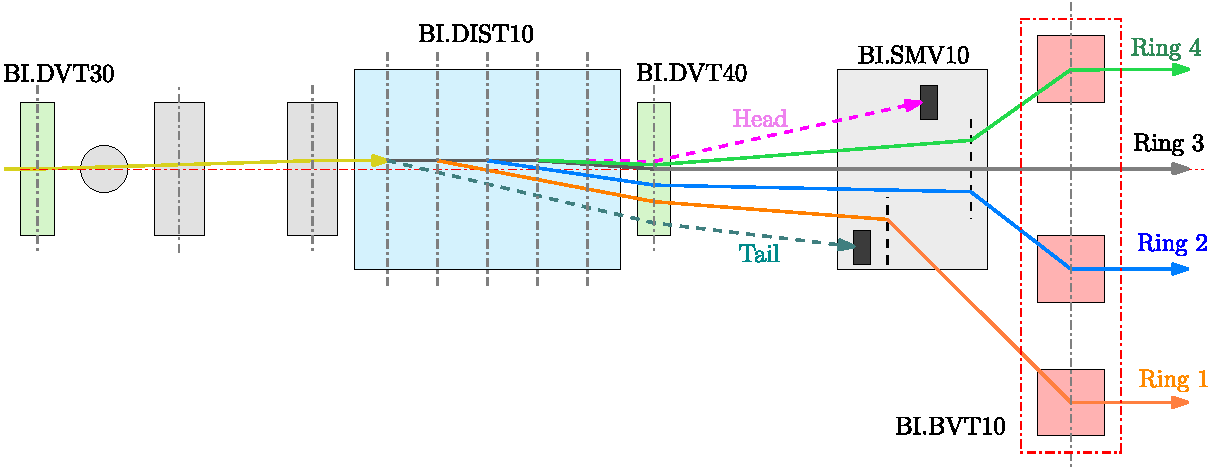
\includegraphics[width=0.9\columnwidth]{Figure_DistributorBeam/InjecLayout.pdf}
    \caption{Schematic representation of the PSB injection line, featuring the DVTs, DIST and SMV vertical separation scheme. }
    \label{fig:Injection}
\end{figure}

During the splitting operation, two spur beams are generated, representing the head and the tail of the beam, which are then intercepted by dedicated dumps. These dump blocks are integrated with the septum magnet as internal devices to the BI.SMV magnet tank.

The beam slices are first sequentially deflected vertically, by fixed field iron magnets (BI.DVT30) before being injected into the beam distributor (BI.DIS) \parencite[][]{ref:DIST}. The BI.DIST system, in combination with the BI.DVT40, deflect the beam sequentially into the different apertures of the BI.SMV10, which further deflects the beam to properly inject it into the four booster rings. 

As briefly discussed in the introduction, Chapter \ref{ch:Introduction}, the pulse coming from Linac4 is a pulsed beam. The distributor timing can be adjusted, providing very big flexibility in terms of beam injection to the PSB. Figure \ref{fig:DistTiming} shows three examples of Linac4 pulse structures and distributor timings. 

When in the following sections we refer to beam turns, we are referring to the number of beam micro-pulses injected into the PSB. 

\begin{figure}[h]
    \centering
    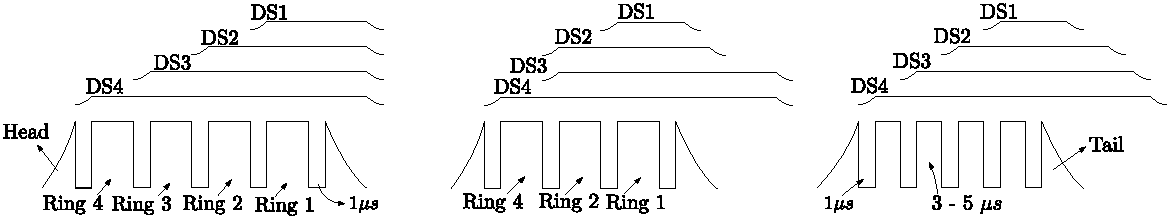
\includegraphics[width=1.0\columnwidth]{Figure_DistTiming/DistTiming.pdf}
    \caption{Possible Linac4 pulse structures and BI.DIS timing. Left: Standard operation with 65 - 100 $\mu s$ injected turns per ring. Center: Operation with 0 turns injected in ring 3. Right: 3-5 injected turns per ring.  }
    \label{fig:DistTiming}
\end{figure}


\section{CEI at CERN PS Booster.}
\label{sec:CEI}

In general, the charge exchange injection (CEI) is performed by stripping two electrons, using thin stripping foils,  from an \hm particle and transforming it into a proton ($p^{+}$).  The closed orbit of the circulating beam is bumped onto the injection orbit, using a set of chicane magnets located around the stripping foil. The fully stripped $p^{+}$ follow the closed orbit of the beam while the partially stripped (\hzz) and the unstripped (\hm) particles are dismissed. 

\begin{figure}[h]
    \centering
    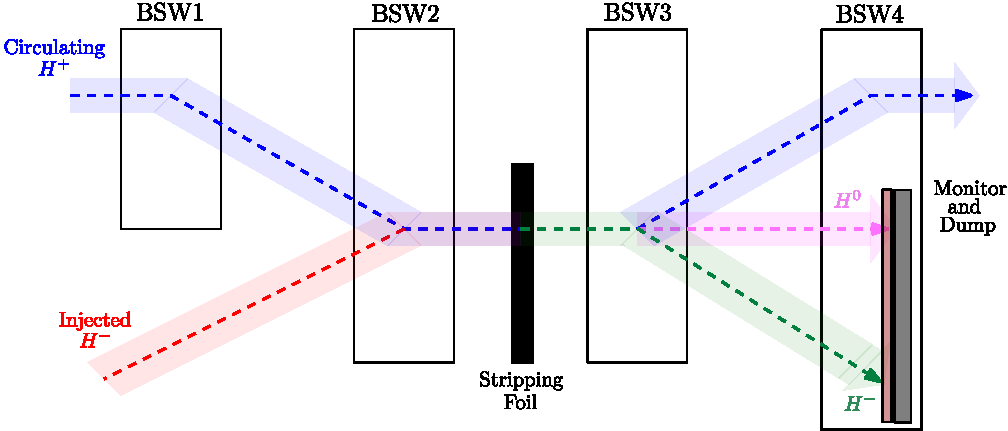
\includegraphics[width=0.75\columnwidth]{Figure_ChargeExchangeSchema/ChargeExSchema.pdf}
    \caption{Schematic representation of PSB \hm Charge Exchange Injection system. }
    \label{fig:SchemaCEI}
\end{figure}

Figure \ref{fig:SchemaCEI} shows a schematic representation of the newly installed CEI system at CERN. The new system comprises, for each of the four booster rings, a stripping foil, a set of four pulsed dipole magnets (BSW) \parencite[][]{ref:BSW} and four horizontal kicker magnets (KSW) \parencite[][]{ref:KSW} (Not depicted in figure \ref{fig:SchemaCEI}). 

The first magnet (BSW1) acts as a septum, generating a high-field region for the circulating beam and a field-free region for the injected \hm beam. It is followed by three bumper magnets (BSW2-4) that help merge the injected beam with the circulating beam. BSW2 and BSW3 are installed at each side of the foil and are identical magnets. BSW4 has an enlarged horizontal gap to accommodate the unstripped particle beam as well as the unstripped particle monitor. Each magnet is powered independently to allow maximum flexibility during operation. 

The stripping foil ( about 20 x 20 mm wide) is made of carbon, with a density of around 200 $\mu g cm^{-2}$. The choice of material and thickness is driven by the stripping efficiency ($> 99 \%$), beam loss and emittance blow up and temperature rise of the foil \parencite[][]{ref:StrippingFoil}. In each of the rings, a set of six foils are available, and can be interchanged thanks to a foil charger and handling system.

\section{$H^{0}H^{-}$  Beam Current Monitors and Dump}


The injection region geometry and the very limited space that is available preclude extraction of the unstripped or partially stripped ions. For that reason, four internal $Ti_{6}Al_{4}V$ dumps (one per ring) were installed downstream of the stripping foil, within the vacuum chamber of the chicane magnet BSW4. Figure \ref{fig:H0H-dump} shows the mechanical design of the dump and figure \ref{fig:H0H-Loc} shows the integration of the dump in the booster ring. 

The geometry of the dump provides an unobstructed passage for the circulating beam during injection, as well as for the injected proton beam, whilst providing optimal protection of the downstream elements by absorbing a few percent of the unstripped beam during regular operation and the full beam in the event of foil failure

\begin{figure}[h]
    \centering
    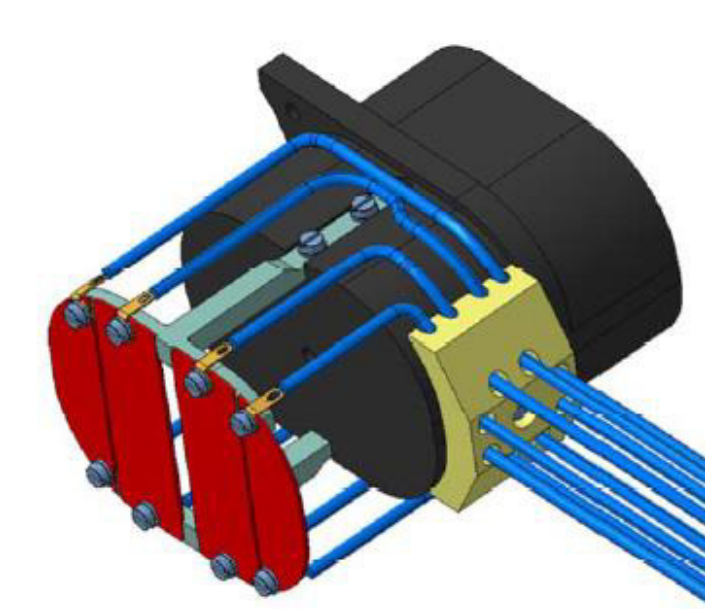
\includegraphics[width=0.45\columnwidth]{Figure_H0H-Monitpor/H0H-.png}
    \caption{Mechanical design of the \hzhm current monitors (red) and Titanium dump (black).}
    \label{fig:H0H-dump}
\end{figure}

An intensity measurement of both, the \hzz and \hm beam particles impacting the dump is required to allow an efficient injection setup, monitor the efficiency of the stripping foil and protect the dump in case of a high-intensity beam impact (by providing an interlock signal in case of stripping foil failure). The \hzhm monitors (represented in red in figure \ref{fig:H0H-dump} and figure \ref{fig:H0H-Loc}) are installed 4 cm upstream of the face of the dump. The distance between the dump and the intensity monitors is sufficient to prevent secondary electrons from the dump from interfering with the signals from the monitors.

\begin{figure}[h]
    \centering
    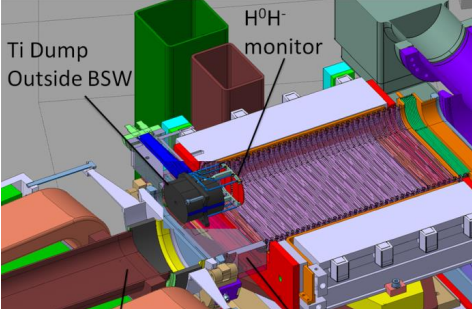
\includegraphics[width=0.6\columnwidth]{Figure_H0H-Monitpor/Instalation.png}
    \caption{Integration of the \hzhm dump (black) and intensity monitor (red plates) in a PSB ring. The purple element is the BSW4 magnet.}
    \label{fig:H0H-Loc}
\end{figure}

The \hzhm intensity monitors consist of four titanium plates: two 22 cm wide central plates and two 18 mm wide external plates with around 1 mm separation between the plates. Having four independent plates allows supplementing the intensity measurements with some beam position information. The two outer plates (with respect to the beam position) are expected to measure \hm particles while the two inner plates are expected to measure the partially stripped \hzz particles. 

Titanium was chosen as the detector material for its low Z (i.e. low activation) and moderate conductivity ($2.34\cdot 10^6 \Omega^{-1} m^{-1}$). This is a good compromise between the high conductivity needed for reading out the deposited charge and the low conductivity required due to the presence of a pulse magnetic field in the BSW4 chamber. The thickness of 1mm guarantees stopping all the stripped electrons and is compatible with the presence of a vertical B-field. 

As shown in figure \ref{fig:H0H-dump} and figure \ref{fig:H0H-Loc}), each monitor plate has two read-out cables (represented in blue). This duplication has been implemented only for hardware redundancy: in the case of cable damage, a second one is immediately available. During operation, only one signal cable per plate is connected to the acquisition system.

\section{Expected signal generation}

The electric signal generated in the plates allows determining the number of \hzz and \hm particles reaching the particle dump, and thus it determines the stripping inefficiency. As explained in chapter \ref{ch:CurrentModeling}, several effects contribute to the charge formation in the plates. In this particular case, the most relevant processes are, charge deposition ($Q_{dep}$) and Secondary emission ($Q_{se}$). 

Table \ref{tab:ExpectedSignal1} summarizes various terms contributing to the plate signal generation per incident particle. Table \ref{tab:ExpectedSignal2} shows the expected values of the signal generated in the \hzhm plates. Due to the two electrons in the \hm particles, a higher signal (per incident particle) is expected in the two right-most plates. SEE in this case will diminish the absolute value of the measured signal, and it will be a non-welcomed effect. Because of the low energy of the SE, the magnetic field of BSW4 is large enough to suppress the SE emission. Thus, the expected charge per incident particle is not greatly affected by SE. More details on this are given in section \ref{sec:SEBSW4}.

% Please add the following required packages to your document preamble:
% \usepackage{multirow}
% Please add the following required packages to your document preamble:
% \usepackage{multirow}
\begin{table}[h]
    \centering
    \begin{tabular}{cccccc}
    \hline
    \multirow{2}{*}{$\eta$} & \multirow{2}{*}{$\mu$} & \multirow{2}{*}{$BS_p$} & \multirow{2}{*}{$BS_e$} & \multirow{2}{*}{$SEY_p$} & \multirow{2}{*}{$SEY_e$} \\
                         &                     &                      &                      &                       &                       \\ \hline
    0.997                & 0.463               & 0                    & 0.5369               & 0.0295                & 0.0779                \\ \hline
    \end{tabular}
    \caption{Necessary values for predicting current generated in \hzhm plates.}
    \label{tab:ExpectedSignal1}
\end{table}

\begin{table}[h]
    \centering
    \begin{tabular}{cccc}
    \hline
    \multicolumn{2}{c}{Q(e/\hzz)} & \multicolumn{2}{c}{Q(e/\hm)} \\
    w. SE        & w.o. SE      & w. SE        & w.o. SE      \\ \hline
    -0.2841      & -0.463       & -0.627       & -0.926       \\ \hline
    \end{tabular}
    \caption{Expected signal generated in \hzhm per incident particle. }
    \label{tab:ExpectedSignal2}
\end{table}

The total number of \hzz and \hm particles depends on the stripping efficiency. In normal operation conditions, during injection, the expected number of \hzz particles is around $2\%$ of the total Linac4 pulse. The expected number of \hm particles is very low $\approx 10^{-4} \%$. Stripping foil degradation is tolerated until the beam dump load reaches a safety limit. Currents larger than $10\%$ of the Linac4 beam pulse generate an interlock signal that stops the particle beam at the source. 

\begin{figure}[h]
    \centering
    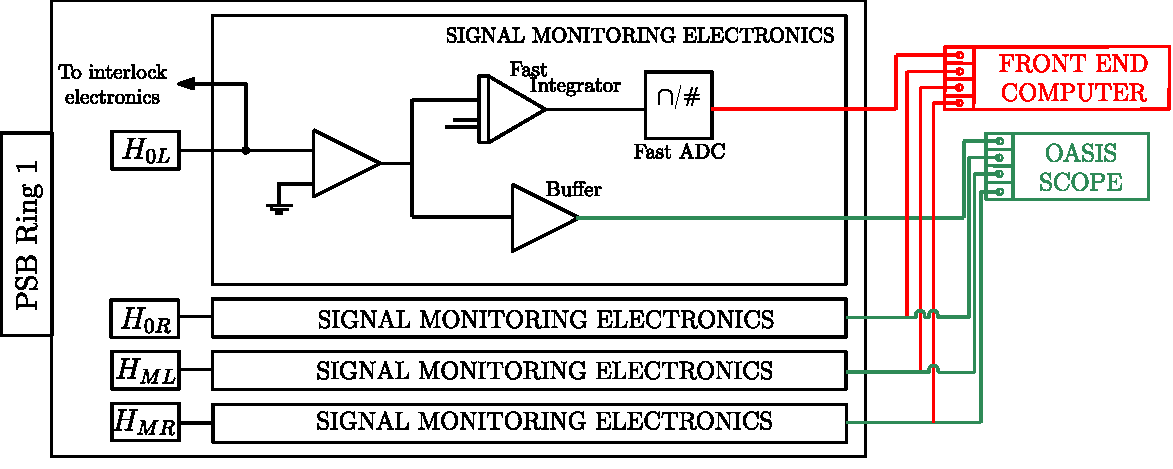
\includegraphics[width=0.9\columnwidth]{Figure_ElectronicSchema/SignalMonitorElec.pdf}
    \caption{Schematic diagram of the signal monitoring electronics.}
    \label{fig:MonitorSchCircuit}
\end{figure}


\section{Monitor Electronics, Layout and funcitonalities}

The electronics for the \hzhm intensity monitors are designed to ensure the continuous measurement of the \hzz and \hm particles and to function as an input to the interlock system that protects the \hzhm dump. For each PSH ring, the electronics for monitoring the 4 plates are embedded into a single VME card. Two main circuits can be found in these cards, the signal monitoring circuit and the interlock circuit. 

\subsection{Signal Monitoring Circuit}

This part of the circuit aims for high sensitivity intensity measurements. A schematic diagram of the electronic circuit can be found in figure \ref{fig:MonitorSchCircuit}. The intensities measured by each plate are fed to a fast amplifier. The amplifier output is connected to an OASIS channel, which gives information on the real-time monitoring of the signal. In paralel, it is also connected to a fast integration system. 

To sample the signal every PSB turn (every $1 \mu s$), the integration is performed using two alternating fast integrators. The timing logic and system response are shown in figure \ref{fig:TimeResponse}. The integrator output is given to a fast ADC, which converts the integrated charges to digital samples. The ADC read-out and the discharge of the integrators take around 120 ns every PSB turn. This limits the length of the beam pulse that can be integrated to a maximum of 780 ns.

\begin{figure}[h]
    \centering
    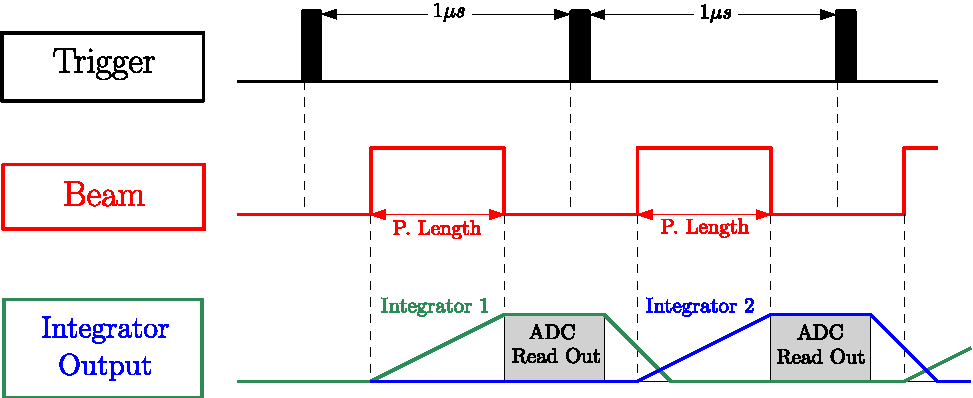
\includegraphics[width=0.8\columnwidth]{Figure_ElectronicSchema/TimeSchema.pdf}
    \caption{Time logic of signal monitoring circuit.}
    \label{fig:TimeResponse}
\end{figure}

\section{Interlock Circuit}

The objective of the interlock circuit is to generate an interlock signal that will protect the \hzhm dump. Figure \ref{fig:InterlockCir} shows the schematic representation of the interlock circuit. In this case, the current coming from each plate is fed to a slow and low-gain amplifier. The outputs from each amplifier serve as parallel input to a slow integrator. The integrator output goes to a comparator, that has the purpose of checking if the total sum is above or below a certain threshold. If the sum is above the thershold, the circuit generates an interlock signal. 

\begin{figure}[h]
    \centering
    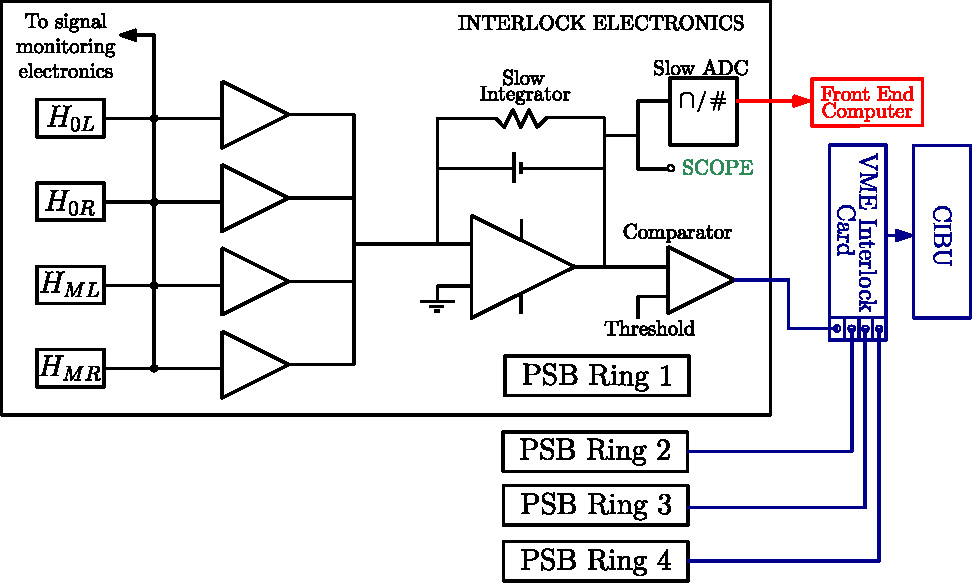
\includegraphics[width=0.8\columnwidth]{Figure_ElectronicSchema/InterlockElectronics.pdf}
    \caption{Schematic diagram of the electronic circuits for the interlock system.}
    \label{fig:InterlockCir}
\end{figure}

The threshold of the comparator can be set via software and was defined after the calibration of the system. If a signal avobe the threshold is detected in any of the rings, the interlock card sends a FALSE signal to the dedicated CIBU (User System to Beam Interlock System Connection) \parencite[][]{ref:CIBU}. The estimated response time between the interlock detection and the beam dumping is around 10 $\mu s$. After each interlock occurrence, the interlock card keeps the FALSE output until the operator uses the RESET command. 

In parallel to the comparator, the analog integrator output is also connected to a slow ADC and to an independent scope connector to allow for different ways of monitoring the interlock electronics. 

\section{Read Out Signals}

As aforementioned, several types of signals from the monitors can be accessed. The usefulness of these signals and how to understand them are discussed in this section. 

\subsection{OASIS signal}
\label{sec:OasisSignal}

The Oasis Scope Signal, or simply the OASIS signal, shows the analog current measured by the plates after a fast amplification. It allows for real-time monitoring. Figure \ref{fig:OasisSignal} shows an example of the signals measured with the OASIS scope. 

\begin{figure}[h]
    \centering
    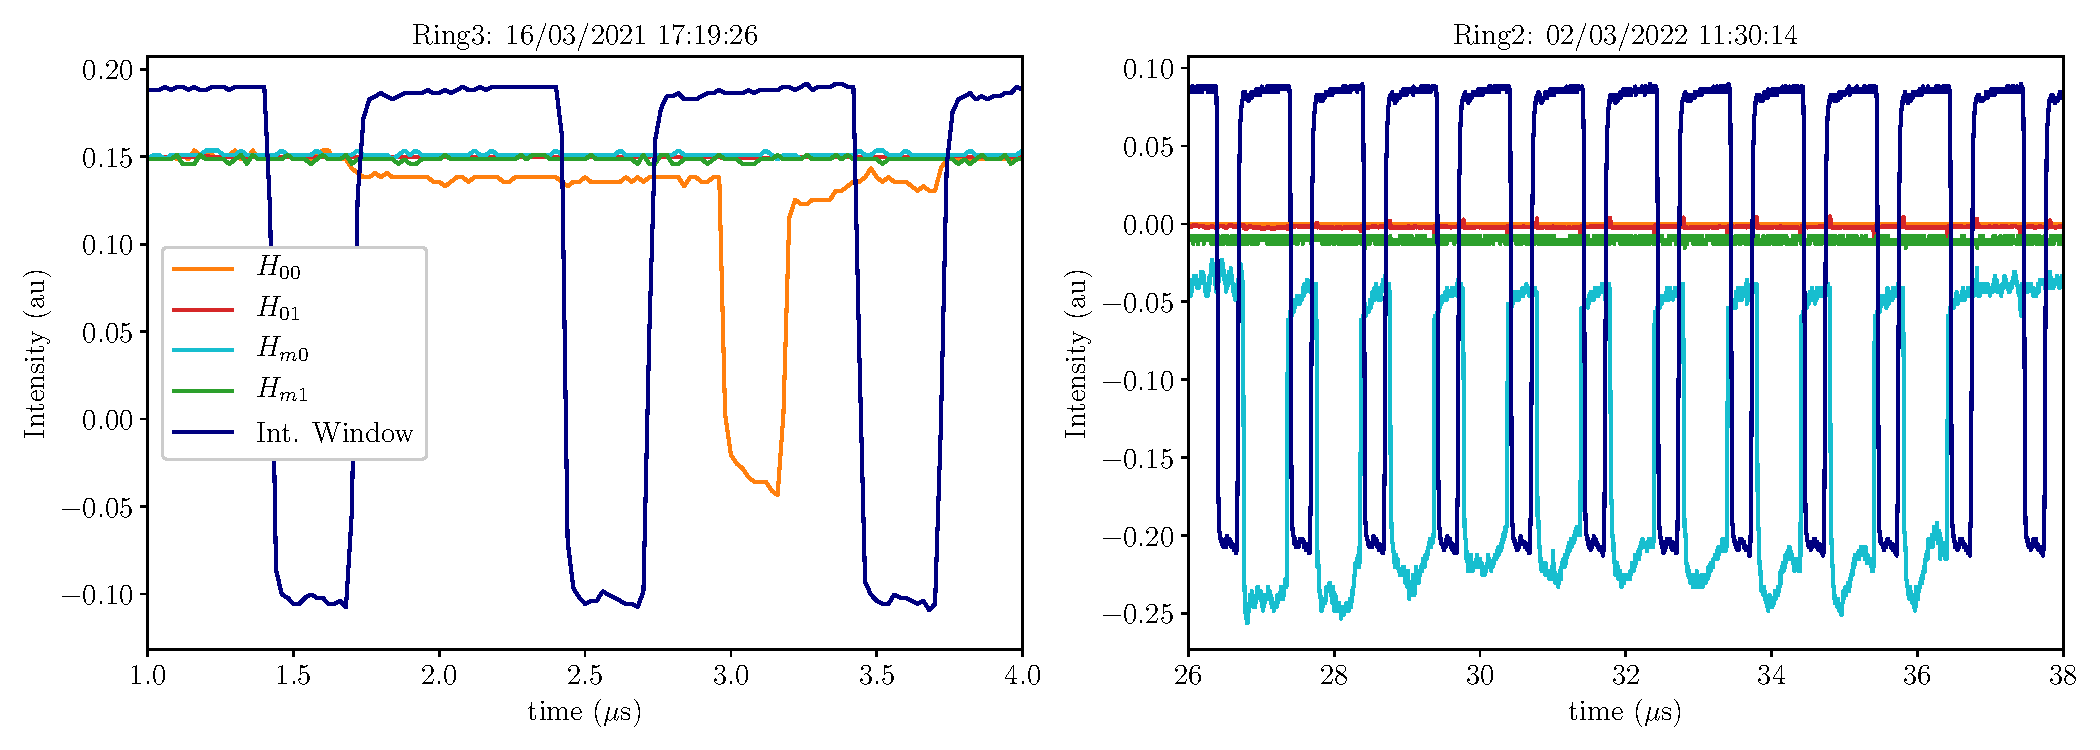
\includegraphics[width=1.0\columnwidth]{Figure_OasisSignals/OasisSignal.pdf}
    \caption{Example of OASIS signals. Left: Single turn, pulse length 200 ns, focused on H0L plate. Right: 10 turns, pulse length 620 ns, focused on HML plate. }
    \label{fig:OasisSignal}
\end{figure}

The figure on the right shows an example of a signal produced by a single bunch injection. On the right, a multiple-turn injection signal is shown. 

In both these pictures, one can observe the signal measured by the four plates. In both cases, the beam of particles was centered on one plate (left: H0L plate; right: HML plate). Depicted in dark blue, one finds the Integrating window signal. Positive readings of this signal mean that the plate signals are being integrated.



\subsection{Plate Signal}

Figure \ref{fig:PlateSignal} shows an example of Plate signal, that is, the signal registered by the front end computer in the signal monitoring circuit. This signal corresponds to the integrated and digitalized OASIS signals. In this figure, different colors indicate different beam conditions. In general, longer beam pulses will result in larger integrated signals (in absolute value) as more charges are being integrated during the same integration window. On the other hand, the larger the number of beam turns, the larger the number of points with integrated charge. 

If we look again at figure \ref{fig:OasisSignal}, one can notice that the Plate signals of the left and right plots would be very different. The left plot would yield a single point with a signal in the plate signal measurement. Whereas the left plot will yield ten points with signal and each one of them with a larger absolute current. 

\begin{figure}[h]
    \centering
    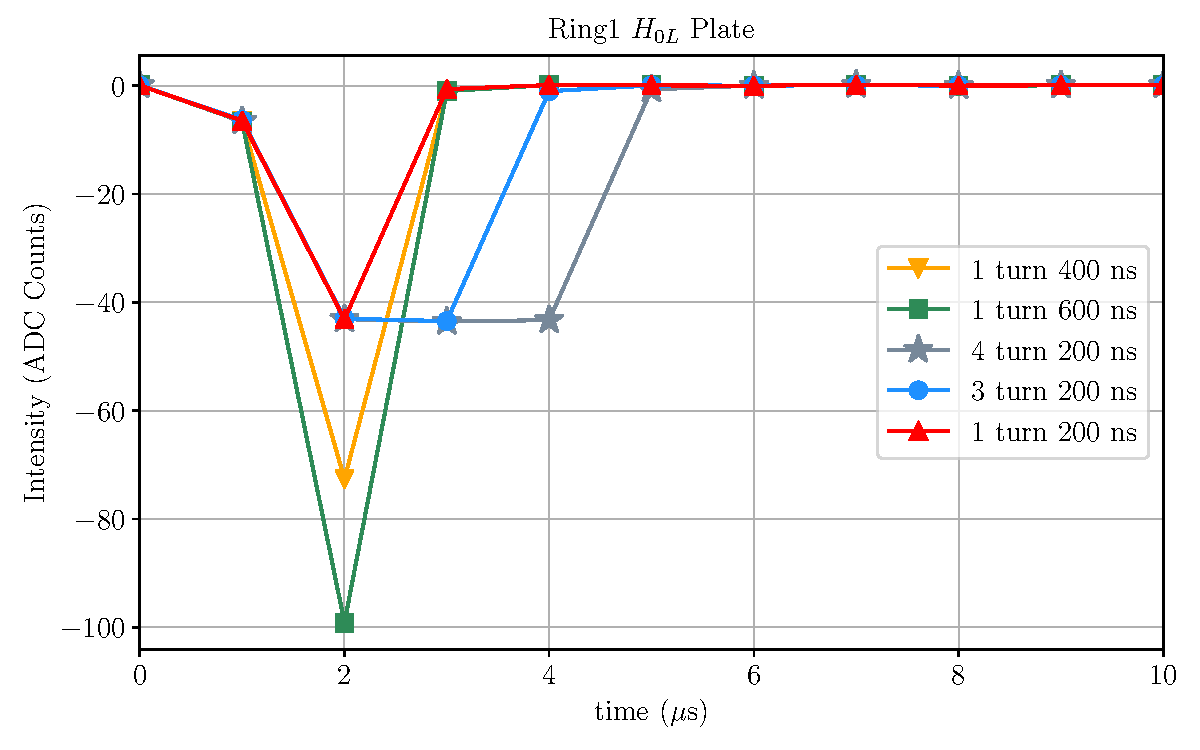
\includegraphics[width=0.7\columnwidth]{Figure_PlateSignal/PlateSignal.pdf}
    \caption{Example of Plate signals for different beam conditions.}
    \label{fig:PlateSignal}
\end{figure}

\subsection{Interlock Signal}

The interlock electronics also had access to an OASIS scope, however, it was rarely used during the measurements. The interlock signal was generally monitored in the front-end computer, after the integrator and ADC. Figure \ref{fig:InterlockSignal} shows some examples of measured interlock signals. Stored in the database is also the signal from the comparator. This is a boolean type signal, indicating whether or not an interlock was generated. In figure \ref{fig:InterlockSignal}, the red signals correspond to cases where the beam was interlocked due to measured signals surpassing the safe threshold. 

\begin{figure}[h]
    \centering
    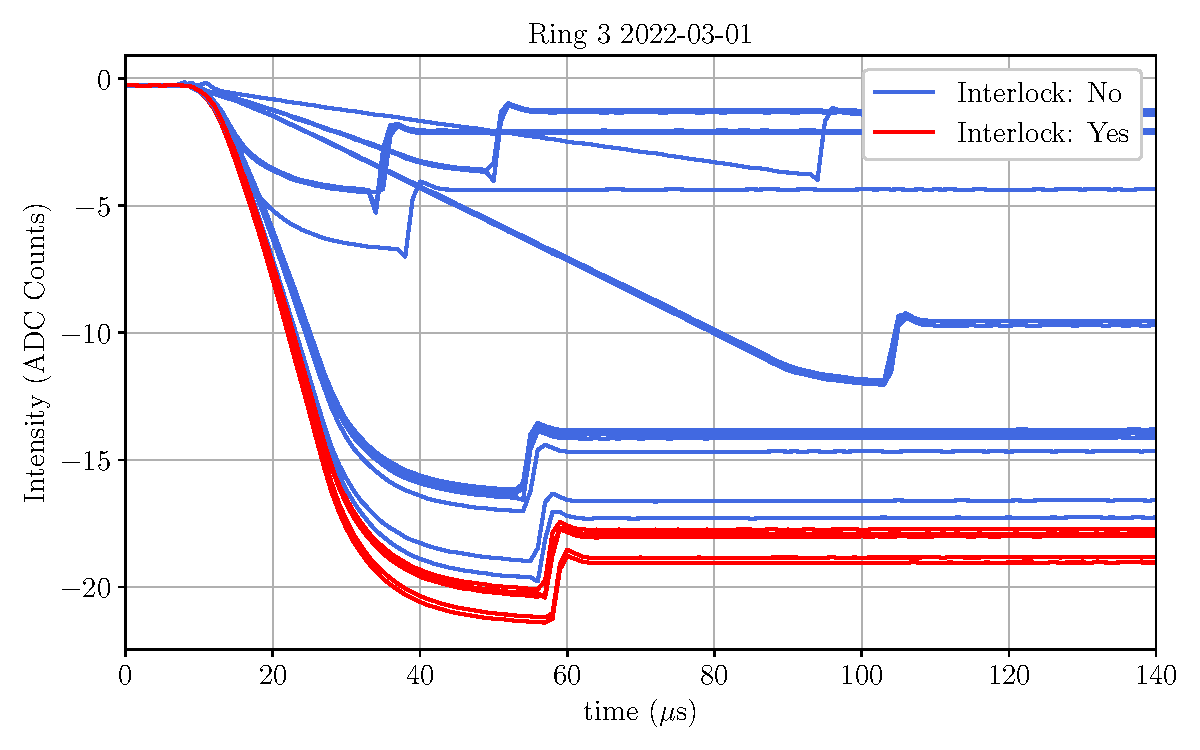
\includegraphics[width=0.7\columnwidth]{Figure_InterlockSignal/InterlockSignal.pdf}
    \caption{Several examples of interlock signals.}
    \label{fig:InterlockSignal}
\end{figure}

\section{Calibration}

\subsection{Objective and Procedure}

The main objective of the \hzhm monitors is to continuously measure the amount of unstripped particles reaching the dedicated dump. The signal generated in the plates is proportional to the number of unstripped particles. However, due to the complicated electronics implementation, the physical meaning of "number of particles" is lost when reading the signals in front-end computers. It was of great importance to recover this information, to fully exploit the potential of the detectors. For that reason, a calibration campaign was launched. 

\begin{figure}[h]
    \centering
    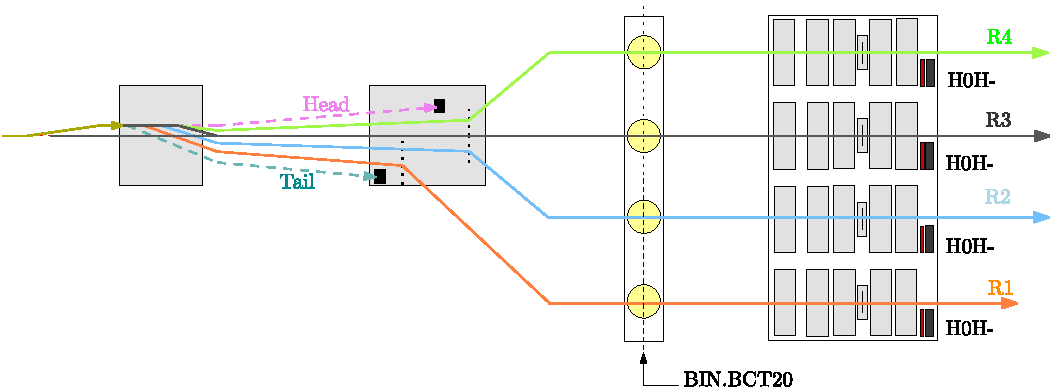
\includegraphics[width=1.0\columnwidth]{Figure_BCTPosition/BctPosSim.pdf}
    \caption{Schematic representation of the BCT (in yellow) location on the beam line. }
    \label{fig:LocationBCTPlate}
\end{figure}

The main objective of this calibration was to obtain a calibration factor ($R_{cal}$) that correlated the ADC counts (Obtained as an output of the electronics) with the total number of particles reaching the dump. This calibration factor was calculated for the Plate Signals, and it had to be calculated independently for all the plates in all the booster rings. 

The calibration was performed with an \hm beam of particles, that is, without stripping foil. In this way, the calibration factor was not dependent on the stripping efficiency of a given foil. Also, the negative nature of the \hm particles facilitated the beam's focusing and guidance. The electronics are optimized for measuring a maximum of $10 \%$ of the Linac4 beam intensity. For that reason, a beam of reduced intensity ($I_{beam} \sim 4$ mA) was used for the calibration.  

An independent measurement of the number of particles reaching the dump was measured with a beam current transformer. The BCTs used for the calibration were placed after the distributor, before the stripping foil. Figure \ref{fig:LocationBCTPlate} shows a schematic representation of the BCTs location on the beamline.

\begin{figure}[h]
    \centering
    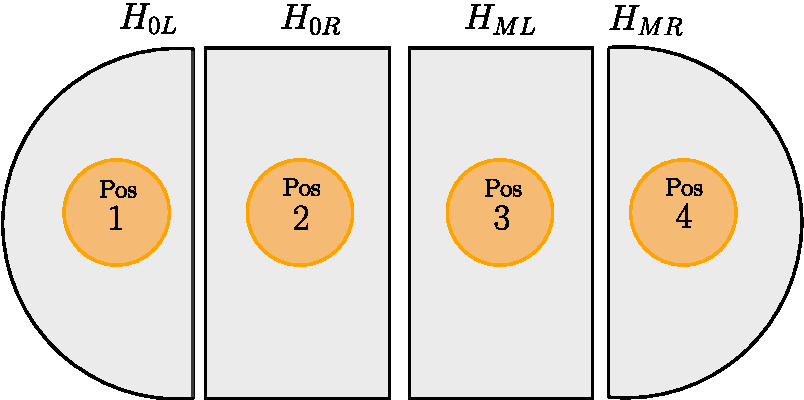
\includegraphics[width=0.5\columnwidth]{Figure_OrderMeasurement/OrderMeas.pdf}
    \caption{Schema of the order followed during the measurements. }
    \label{fig:MeasSeq}
\end{figure}

The calibration measurements were taken in several different days, and under different beam conditions. However, the measurement procedure was always the same. The beam of particles was focused individually in each plate, from "left" to "right", thanks to BSW3 and BSW4 and other kicker magnets ( see measurement sequence indicated in figure \ref{fig:MeasSeq}). 

The calibration factor was calculated by taking the integral of the plate signal and comparing the results with the total number of charges measured by the BCT in each case. A mathematical description of this calibration facture can be written as: 

\begin{equation}
    R_{cal}\left[\frac{Charge}{ADCcounts}\right] = \frac{Signal BCT}{Signal Plate}\cdot C_{f}
\end{equation}

Here, $C_f$ stands for correction factor, and it will be covered in the next section. A sample of the plate signal measurements, taken during a scan at Ring2, are shown in figure \ref{fig:PlateSignalExample}. In this case, a beam pulse of 200 ns and 1 Booster turn were used for the calibration. From this figure, one can see that the four plates seem to give very similar measurements. To compare the results with the BCT measurements, the integral of this signal along the shaded area was calculated.  

\begin{figure}[h]
    \centering
    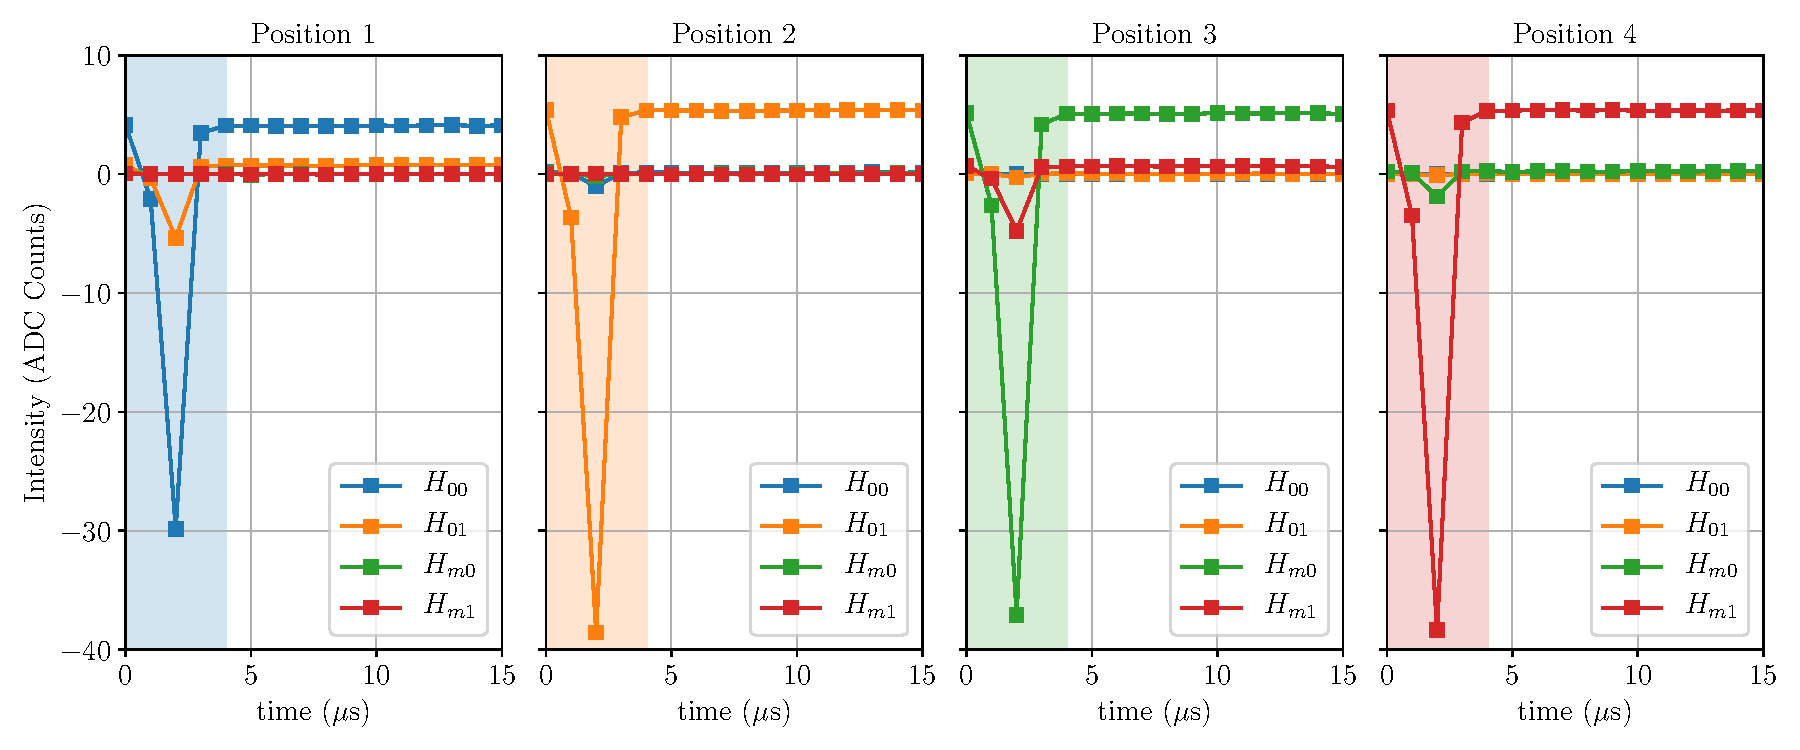
\includegraphics[width=1.0\columnwidth]{Figure_ExampleCalCalculation/ExampleScan.pdf}
    \caption{Example of measurement taken during a scan in Ring 2. Shaded area, integration window for the total charge calculation. }
    \label{fig:PlateSignalExample}
\end{figure}

\subsection{Correction Factor}

To properly compare the measurements taken with the different plates to the BCT measurements, some corrections must be applied. These corrections are: offset corrections, beam displacement effects and tail/head beam effects. 

\subsubsection{Background Correction}

The plate signal measurements seem to suffer beam-line displacements when a non-negligible current is measured. This is corrected by subtracting the average of the measured signal after the beam passage. See figure \ref{fig:BackCorrection} for an example of background subtraction. In this example, a 200 ns beam pulse with 4 Booster turns was measured. The beam of particles was focused on the $H_{0L}$ plate. The shaded area indicates the part of the signal that was used for background corrections. If a beam of particles with a very number of turns was measured, the background window was adapted correspondingly. 

\begin{figure}[h]
    \centering
    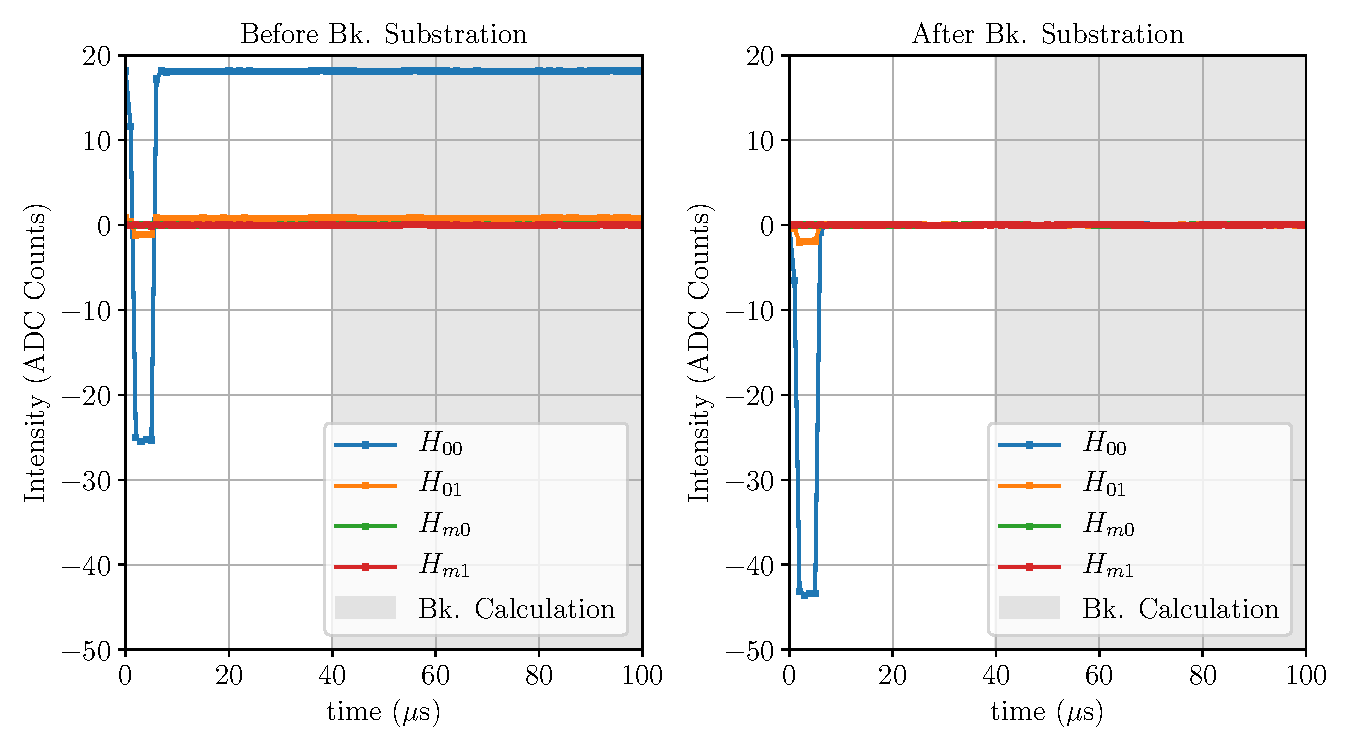
\includegraphics[width=0.85\columnwidth]{Figure_BeforeAfterBackground/BeforeAfterBk.pdf}
    \caption{Example of background correction. Left: Before correction. Right: After correction}
    \label{fig:BackCorrection}
\end{figure}

\subsubsection{Beam displacement effects}

The calibration was done for each plate at a time, by focusing the beam on each of them individually. However, in some cases, we were unable to fully focus the beam on a single plate. See figure \ref{fig:BeamDisplacement} for an example of a not fully centered beam. In this case, the beam was supposedly centered on H0L, however, a small current intensity could be measured on H0R. because the intensity measured by the BCTs os the total intensity of the beam, one can't compare directly the signal measured by a single plate with the BCT signal. First, a correction factor ($C_{f}$) was applied: 

\begin{equation}
    C_f = \prod_{m}  \cdot \frac{H_n}{H_n + H_m}
\end{equation}

With $H_{n}$ being the calculated integral on plate n, and $H_{m}$ the calculated signal on adjacent plates. This might be an overly complicated way of compactly writing a mathematical expression for the $C_{f}$. As an example, one could calculate the $C_{f}$ of figure \ref{fig:BeamDisplacement} as follows:  

\begin{equation}
    C_f = \frac{H_{0L}}{H_{0L}+H_{0R}} = \frac{-181.033}{-181.033-7.930} = 0.958
\end{equation}

It is important to note that for the two central plates one might need to calculate a correction factor for the two adjacent plates. 

\begin{figure}[h]
    \centering
    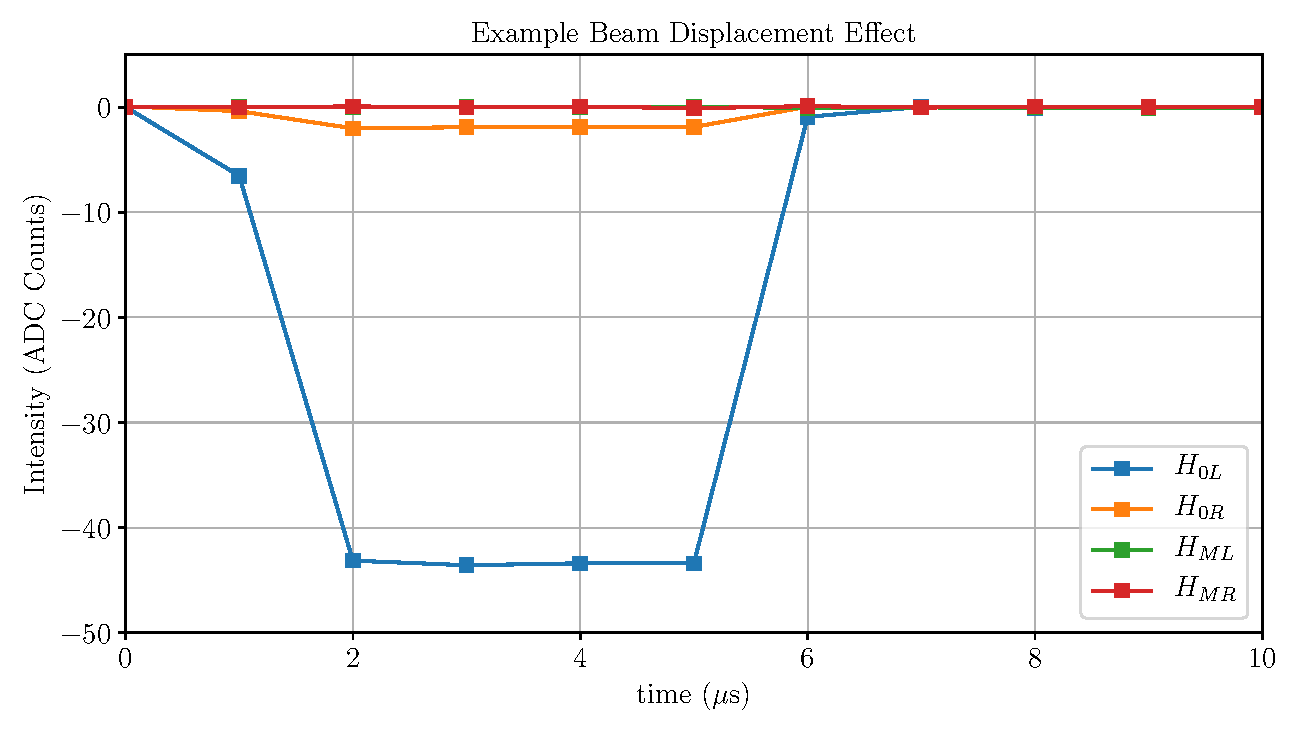
\includegraphics[width=0.75\columnwidth]{Figure_BeamDisplacement/BeamDispEff.pdf}
    \caption{Example of beam displacement effect, for a 4 turn, 200 ns beam. }
    \label{fig:BeamDisplacement}
\end{figure}

\subsubsection{Tail/Head Beam Effects}

In ideal conditions, the bunched beam of particles has a rectangular current profile in the longitudinal space \parencite[][]{ref:headtail}. However, being the world not ideal, we could observe some variations from this rectangular shape. We will call the head of the beam those particles that arrive before the particle bunch and the tail of the beam to those particles arriving after the expected bunch. 

Figure \ref{fig:HeadTailBCT} shows an example of intensity measurement taken with BCT20 at Ring3. The BCT signal that we use for calculating the calibration factor corresponds to the integral inside the orange window of this signal. From this figure, one can see that the beam head is outside the assigned integration area. 

\begin{figure}[h]
    \centering
    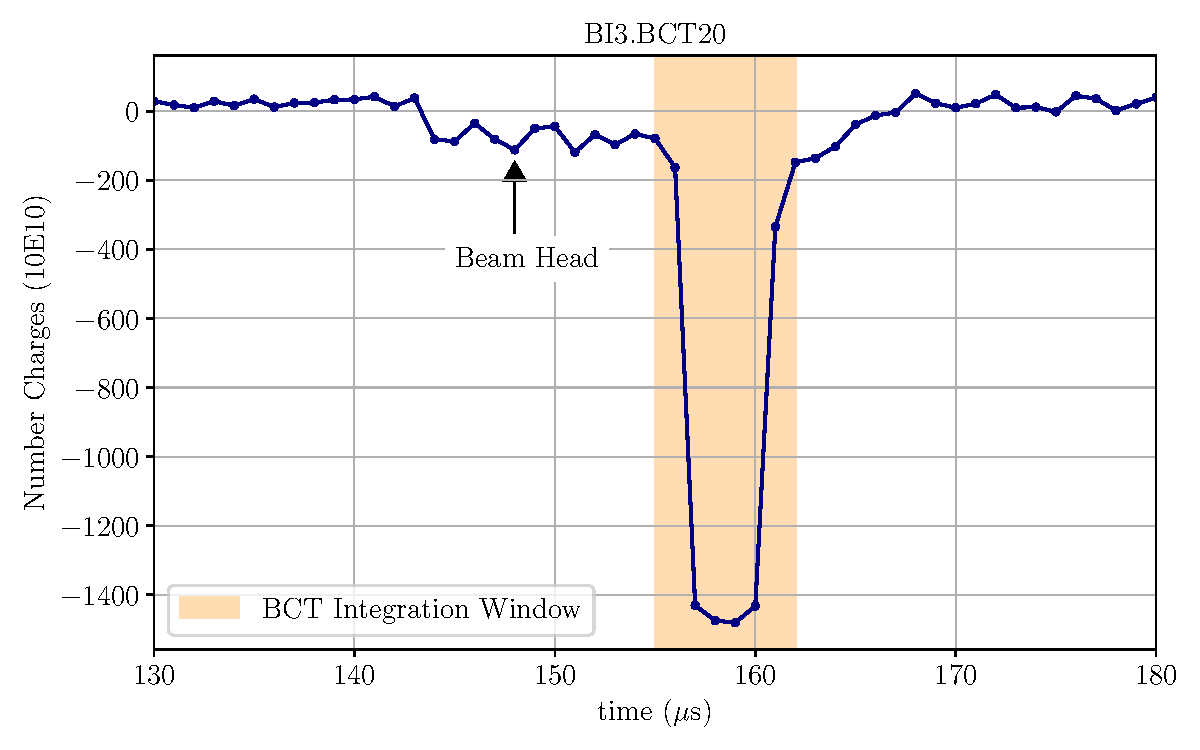
\includegraphics[width=0.75\columnwidth]{Figures_BeamTailEffect/BCT_HeadTail.pdf}
    \caption{Example of BCT measurements, number of charges with time. }
    \label{fig:HeadTailBCT}
\end{figure}

To visualize the head tail effects on the \hzhm monitors we need to look at the OASIS signal. Figure \ref{fig:HeadTailPlate} shows an example of OASIS signal measured by the plates (left) and its corresponding Plate Signal (right). In the OASIS signal, one can easily identify the beam signal as well as the head and tail of the beam. In section \ref{sec:OasisSignal} we explained that whenever the integration window signal was positive, the signals measured by the plates were being integrated. This means that, in the digitalized plate signal, the points immediately before and after the beam pulse correspond to the integral of the beam head and tail (indicated in red in figure \ref{fig:HeadTailPlate} right.). Before calculating the integral of the Plate signal, and compare it to the BCT, it is necessary to correct these points. In figure \ref{fig:HeadTailPlate} (right) one can observe the results of this correction in the plate signal. This effect was particularly important in Ring 4.

\begin{figure}[h]
    \centering
    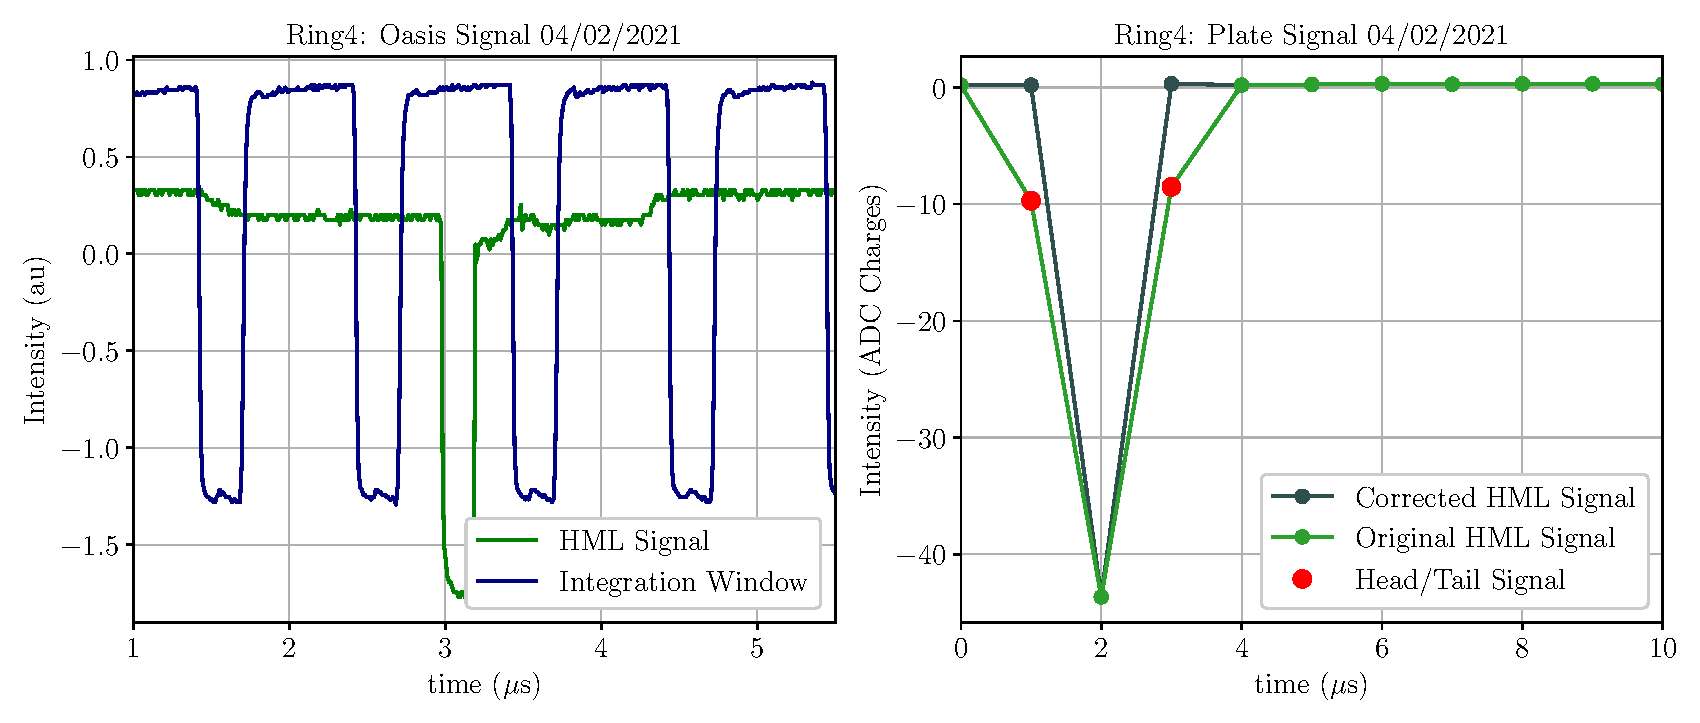
\includegraphics[width=1.0\columnwidth]{Figures_BeamTailEffect/Plate_HeadTail.pdf}
    \caption{ OSIS (left) and Plate signal (right) for a measurement particle beam centered in HML plate. Non-negligible head/tail effects.}
    \label{fig:HeadTailPlate}
\end{figure}

\subsection{Results}

\subsubsection{200 ns, 1 Injected turn}

The calibration was performed with different beam conditions, different pulse lengths (from 200 ns - 700 ns) and a different number of booster injected turns (1 turn - 4 turns). The measurements of the beam intensity remained very stable during all the measurements, with an intensity variation of $2\%$. Figure \ref{fig:IntensityMeas} shows the measured beam intensity in the different rings during the measurements of a 1 turn, 200 ns beam pulse. 

\begin{figure}[h]
    \centering
    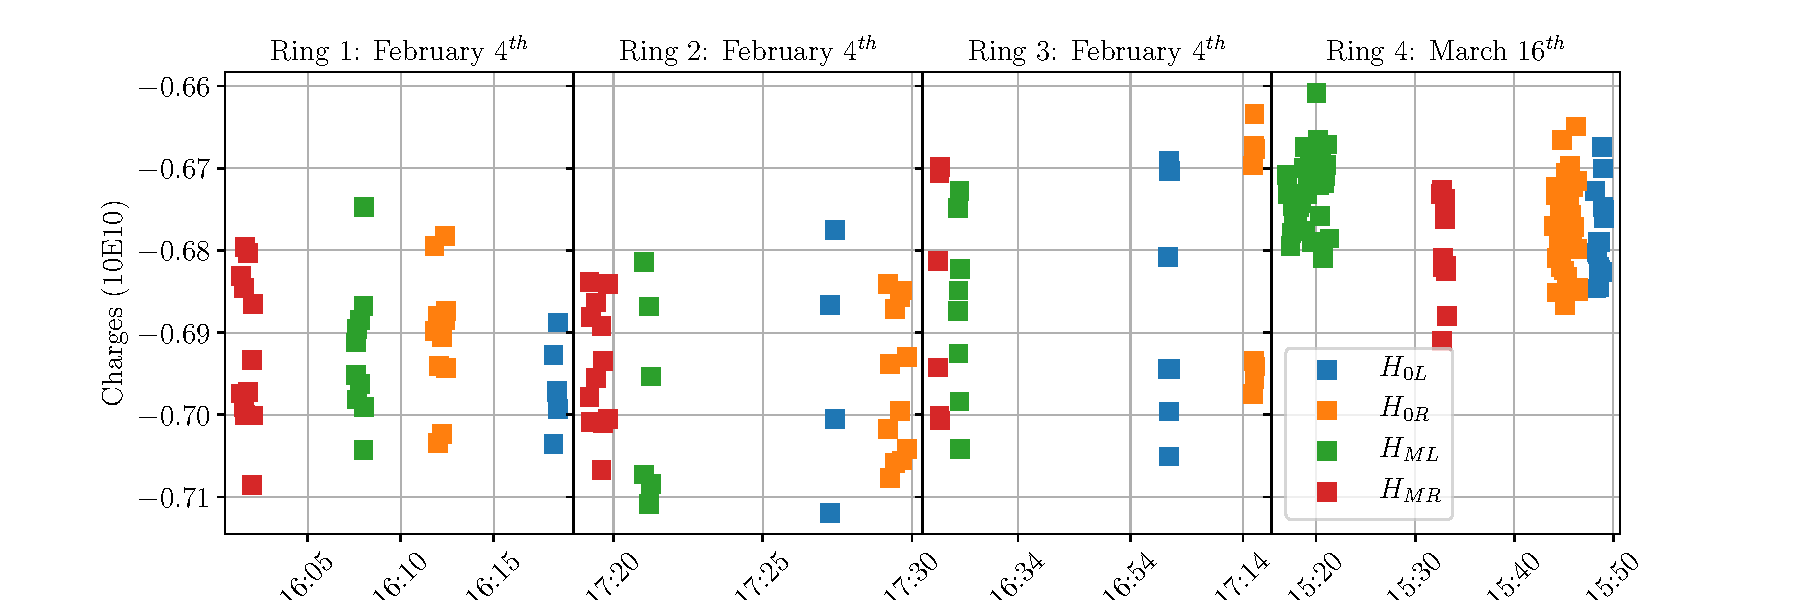
\includegraphics[width=1.0\columnwidth]{Figure_ResultsBCTStability/BctStability.pdf}
    \caption{ Number of charges measured by BCTs during the plate signal calibration. For 1 injected beam turn and 200 ns beam pulse. }
    \label{fig:IntensityMeas}
\end{figure}

Table \ref{tab:CalFac} shows a summary of the calibration factor results for 1 turn, 200 ns particle beam. From these results, one can observe that all the integrated plate signals are negative, and around -43.617(10) ADCcounts. With H0R plate in Ring 2 being the only outlier. Unfortunately, due to lack of time, this measurement could not be repeated. The correction factor ($C_f$), which accounted for beam displacement effects, are all well above 80$\%$, indicating that the beam was properly centered in the calibration plate. All the calibration factors in this case, agree around a value of $R = 1.521(24)\cdot 10^8$ (Charges/ADC count), with H0R in Ring2 again as an outlier. 


\begin{table}[h]
    \centering
    \begin{tabular}{cccccc}
    \hline
                            &                & $\mathbf{H_{0R}}$         & $\mathbf{H_{0L}}$        & $\mathbf{H_{MR}}$         & $\mathbf{H_{MR}}$         \\ \hline
    \multirow{3}{*}{\textbf{Ring 1}} & Int & -43.215(90) & -43.932(69) & -43.763(42) & -43.675(29) \\
                            & $C_f$              & 0.952(1)    & 0.998(2)    & 0.957(1)    & 1.0         \\
                            & R              & 1.534(10)   & 1.568(15)   & 1.514(17)   & 1.585(20)   \\ \hline
    \multirow{3}{*}{\textbf{Ring 2}} & Int & -33.588(31) & -43.925(28) & -42.368(16) & -43.748(51) \\
                            & $C_f$              & 0.844(3)    & 0.971(2)    & 0.892(4)    & 0.954(3)    \\
                            & R              & 1.745(38)  & 1.539(20)   & 1.470(24)   & 1.514(15)   \\
                            \hline
    \multirow{3}{*}{\textbf{Ring 3}} & Int & -43.955(15) & -23.42(74)${}^{(1)}$ & -43.814(80) & -44.190(16) \\
                            & $C_f$              & 0.9508(2)   & 0.535(16)${}^{(1)}$  & 0.9677(7)   & 1.0         \\
                            & R              & 1.482(29)   & 1.565(31)${}^{(1)}$  & 1.517(22)   & 1.552(29)   \\ \hline
    \multirow{3}{*}{\textbf{Ring 4}} & Int & -43.367(50) & -43.638(48) & -           & -43.429(32) \\
                            & $C_f$             & 0.932(1)    & 0.967(1)    & -           & 0.955(1)    \\
                            & R              & 1.459(8)    & 1.502(1)    & -           & 1.497(13)   \\ \hline 
    \end{tabular}
    \caption{Summary of calibration factor results for 1 turn, 200 ns particle beams. The rows Int refers to the integral of the plate signal, with units of ADC counts. ${}^{1}$ was calibrated with the particle beam centered in between $H_{0R}$ and $H_{0L}$, thus the 0.535 calibration factor. }
    \label{tab:CalFac}
\end{table}

\subsubsection{Beam Pulse Length and Number of Injected turns}

Because the calibration factor is calculated by normalizing the signal in the plate with the BCT signal, a change in the beam pulse length or the injected number of turns should not affect the value of the calibration factor.  This assumption was carefully cross-checked.
Figure \ref{fig:PulseLenghtNturns} left, shows the charges measured by the BCT for different beam pulse lengths (from 200 ns to 700 ns), and a constant 1 injected turn. In this figure, one can observe four groups of points. A longer beam pulse implies a larger number of beam charges in each pulse, and thus a larger negative signal. 

\begin{figure}[h]
    \centering
    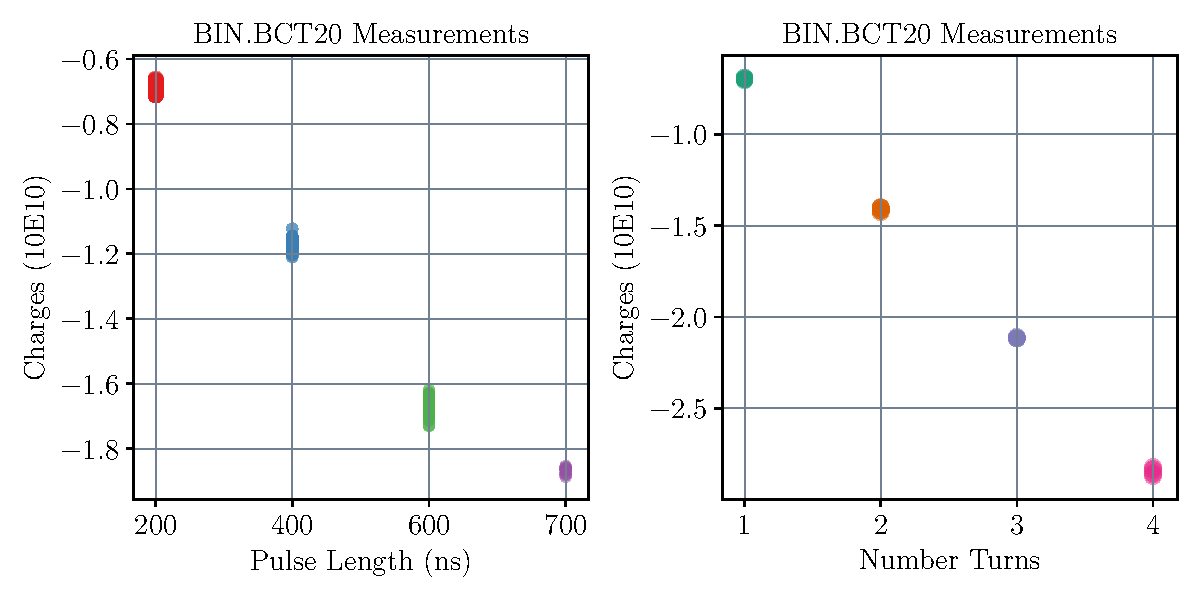
\includegraphics[width=1.0\columnwidth]{Figure_BCT_PulseLength/BCT_TurnPulse.pdf}
    \caption{Number of charges measured by the BCT during Ring1 calibration. Left: for 1 injected beam turn, different beam pulse lengths. Right: For a 200 ns beam pulse length, a different number of turns was injected.}
    \label{fig:PulseLenghtNturns}
\end{figure}

Similarly, the BCT measurements for a 200 ns beam pulse length and various injection turns are shown in figure \ref{fig:PulseLenghtNturns} right. Also, in this case, a larger number of injected turns induces a larger negative signal. 

This tendency was also observed in the Plate signals, however, differences in the pulse length - measured intensity slope (or number of turns - measured intensity slope) between the BCT and the Plate signal measurements, yielded a non-negligible linear dependency of the calibration factor with this properties. Figure \ref{fig:CalfacPlenNturn} shows the calibration measured calibration factor as a function of beam pulse length (left) and number of injected turns (right).

The issue was attributed to mismatches with the integration windows. The maximum length of the integration window for the plate signal is around 650 ns. If the pulse length is longer than that, part of the pulse is not integrated, resulting in a larger calibration factor. In normal operations, beam pulse lengths should not be larger than 600 ns. 

A clear physical explanation for the linear dependency of $R_{cal}$ with the number of turns was not found. Nevertheless, the relative error induced due to this linearity is smaller than $1.5 \%$, so it was not considered to be a critical source of error. 

\begin{figure}[h]
    \centering
    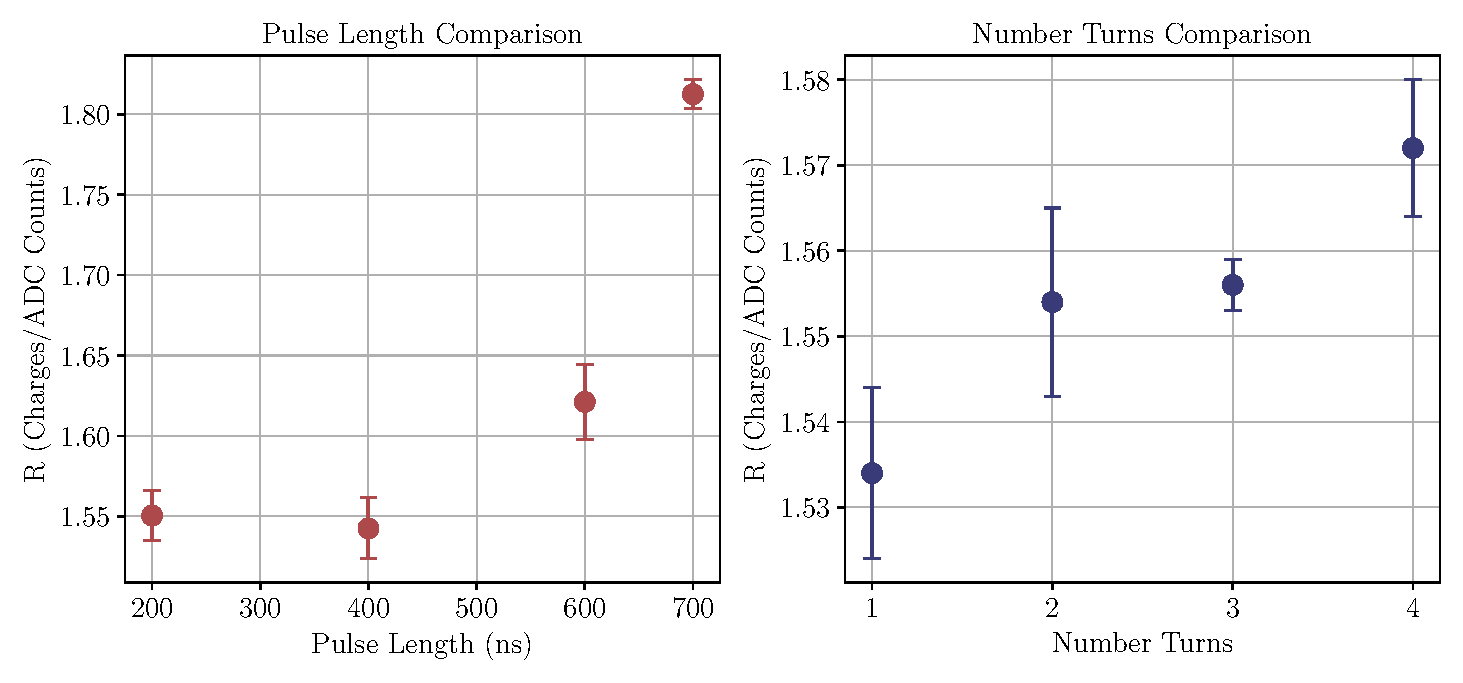
\includegraphics[width=1.0\columnwidth]{Figure_CalFactorLinearity/CalfacLin.pdf}
    \caption{Comparison of calibration factors calculated for different beam conditions.  Left: for 1 injected beam turn, different beam pulse lengths. Right: For a 200 ns beam pulse length, a different number of turns was injected. }
    \label{fig:CalfacPlenNturn}
\end{figure}

\subsubsection{Effects of BSW4 magnetic field}
\label{sec:SEBSW4}

As indicated in section \ref{sec:CEI}, the \hzhm monitors are placed inside BSW4 magnetic field, e.e. they are exposed to a constant magnetic field of $\sim 0.18 $ T. During calibration, BSW4 was able to be turned on and off at will. This allowed us to study the effects this magnetic field had on the intensity measurements. Without the magnetic field of BSW4, the beam could not be focused on the HMR, HML plates. 

The intensity of the magnetic field is enough to suppress the SE produced during the interaction of the particle beam and the plate surface. As explained in chapter \ref{ch:CurrentModeling}, SE will provide a positive contribution to the total current. This means, that if there is secondary emission, a smaller signal (in absolute value) is registered by the plates. A smaller signal in the plates implies a larger calibration factor, as the BCT measurement will remain the same independently of the BSW4 state. 

\begin{figure}[h]
    \centering
    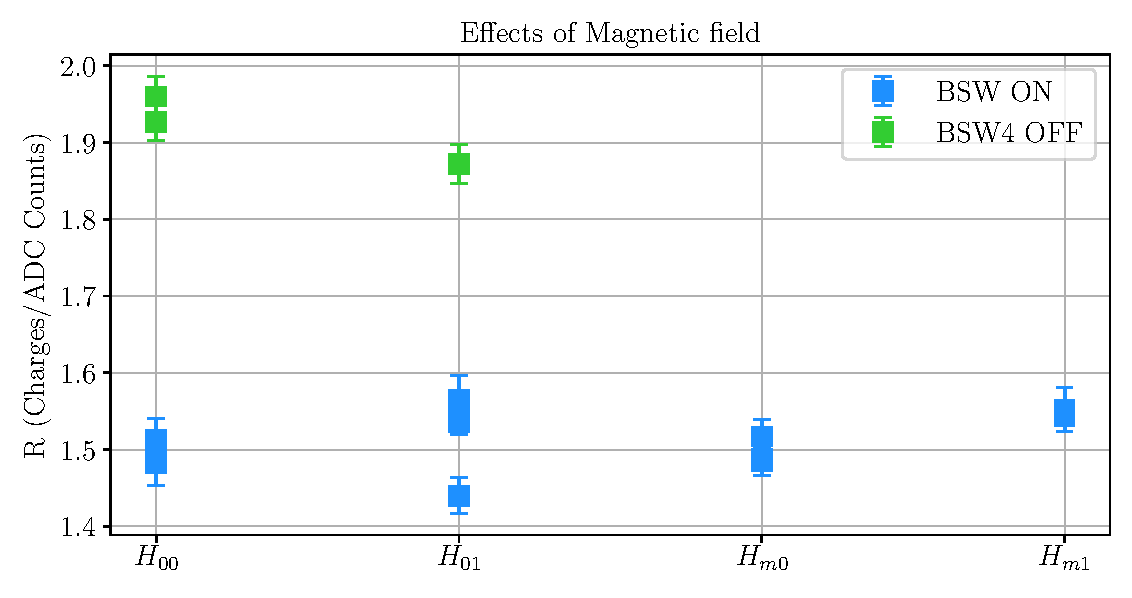
\includegraphics[width=0.75\columnwidth]{Figure_MagneticFieldCompa/MagnetEffect.pdf}
    \caption{Comparison calibration factor with and without BSW4 magnetic field.}
    \label{fig:MagneticFieldEffect}
\end{figure}

This effect can be observed in figure \ref{fig:MagneticFieldEffect}, where the comparison of the calibration factors calculated with and without BSW4's magnetic field is shown. The average calibration factor with magnetic field is $R_{cal} = 1.51(2)$ whereas the calibration factor without magnetic field is $R_{cal} = 1.91(2)$. This is a $26.49 \%$ difference between the values. From table \ref{tab:ExpectedSignal2} we can observe, that the predicted values for the charge formation in the plates, with and without SE, differ a $32.28 \%$, which is consistent with the measured results. 

In normal operation conditions, the magnetic field of BSW4 is always present. 

\subsubsection{Results Summary}

Figure \ref{fig:SummaryR} shows the summary of the calibration factor measurements. It comprises the measurements taken in all the plates, all the rings, and different beam conditions. From this figure, one can observe that all the measurements seem to agree on a calibration factor of: 

\begin{equation}
    R_{cal} = 1.56 \pm 0.033 \cdot 10^8 \hspace{0.4cm} \left(\frac{Charges}{ADC counts}\right)
\end{equation}

With a confidence error smaller than $3.5\%$. This calibration factor was included in the software specifications of the \hzhm monitors so that currently the total number of unstripped particles is continuously available. After the detailed calibration, the monitors became operational. They have continuously been used since April 2021, and have proven to be a really valuable part of the machine operation. 

\begin{figure}[h]
    \centering
    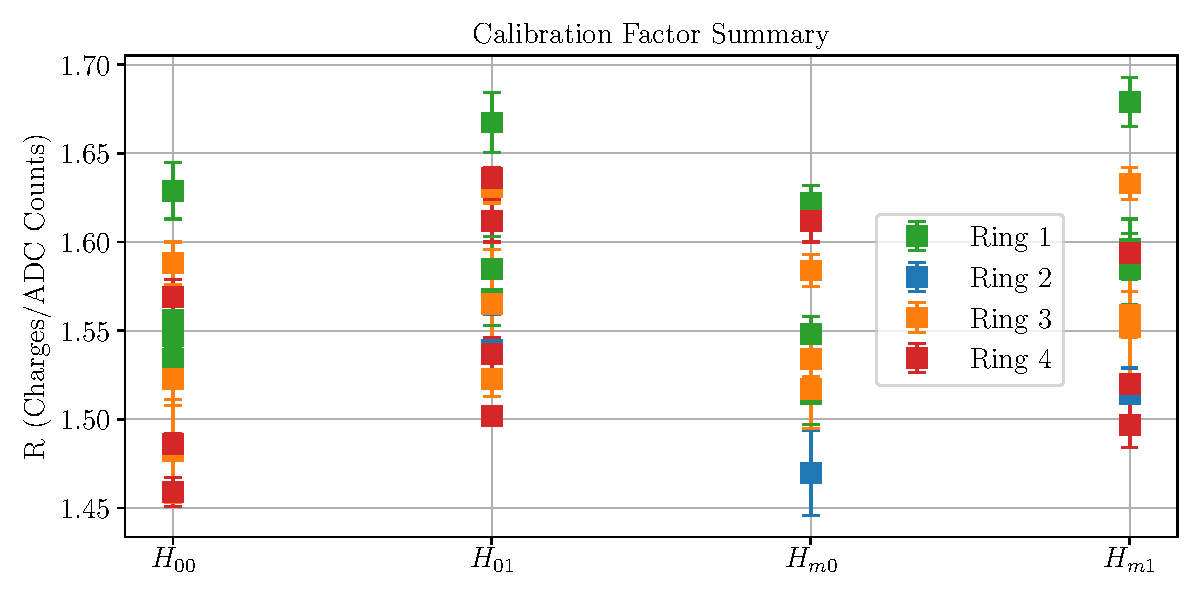
\includegraphics[width=0.9\columnwidth]{Figure_MeasurementSummary/CalSummary.pdf}
    \caption{Summary of the calibration factor measurements.}
    \label{fig:SummaryR}
\end{figure}

\section{Stripping Inneficiency Calculations}

Once calibrated, these detectors could be used to monitor changes in the stripping inefficiency. On April 2021, a dedicated set of stripping foil tests was performed. The objective of the measurement was to test the six stripping foils installed in the loader or Ring3 and to observe their behavior under different beam conditions. Table \ref{tab:SfType} shows the characteristics of the different foils tested during the measurements. 

\begin{table}[h]
    \begin{tabular}{cccc}
    \hline
    \multicolumn{1}{l}{\textbf{Foil Number}} & \textbf{Type} & \textbf{Weight} & \textbf{Description}            \\ \hline
    1-4                                      & XCF-200       & 200 mu g cm2    & Arc evaporated amorphous Carbon \\
    2-5                                      & MLG-250       & 240 mu g cm2    & Multilayer Graphene             \\
    3-6                                      & GSI-200       & 200 mu g cm2    & Arc evaporated amorphous Carbon \\ \hline
    \end{tabular}
    \caption{Characteristics of the measured stripping foils. }
    \label{tab:SfType}
\end{table}

Figure \ref{fig:StrippingIneff} shows the values of the stripping inefficiencies as a function of time, calculated with the \hzhm monitors. Due to the time resolution of the detector, the stripping inefficiency was calculated every microsecond. However, for the sake of visualization, only some of those points have been represented. 

The stripping foils in the loader are assigned a number. In figure \ref{fig:StrippingIneff} the black line represents the stripping foil number, meaning which stripping foil was inserted at each time. The abrupt changes in this line indicate a change in the stripping foil. One can observe that changes on the stripping foil are very much aligned with the changes on the measured stripping inefficiency. 

\begin{figure}[h]
    \centering
    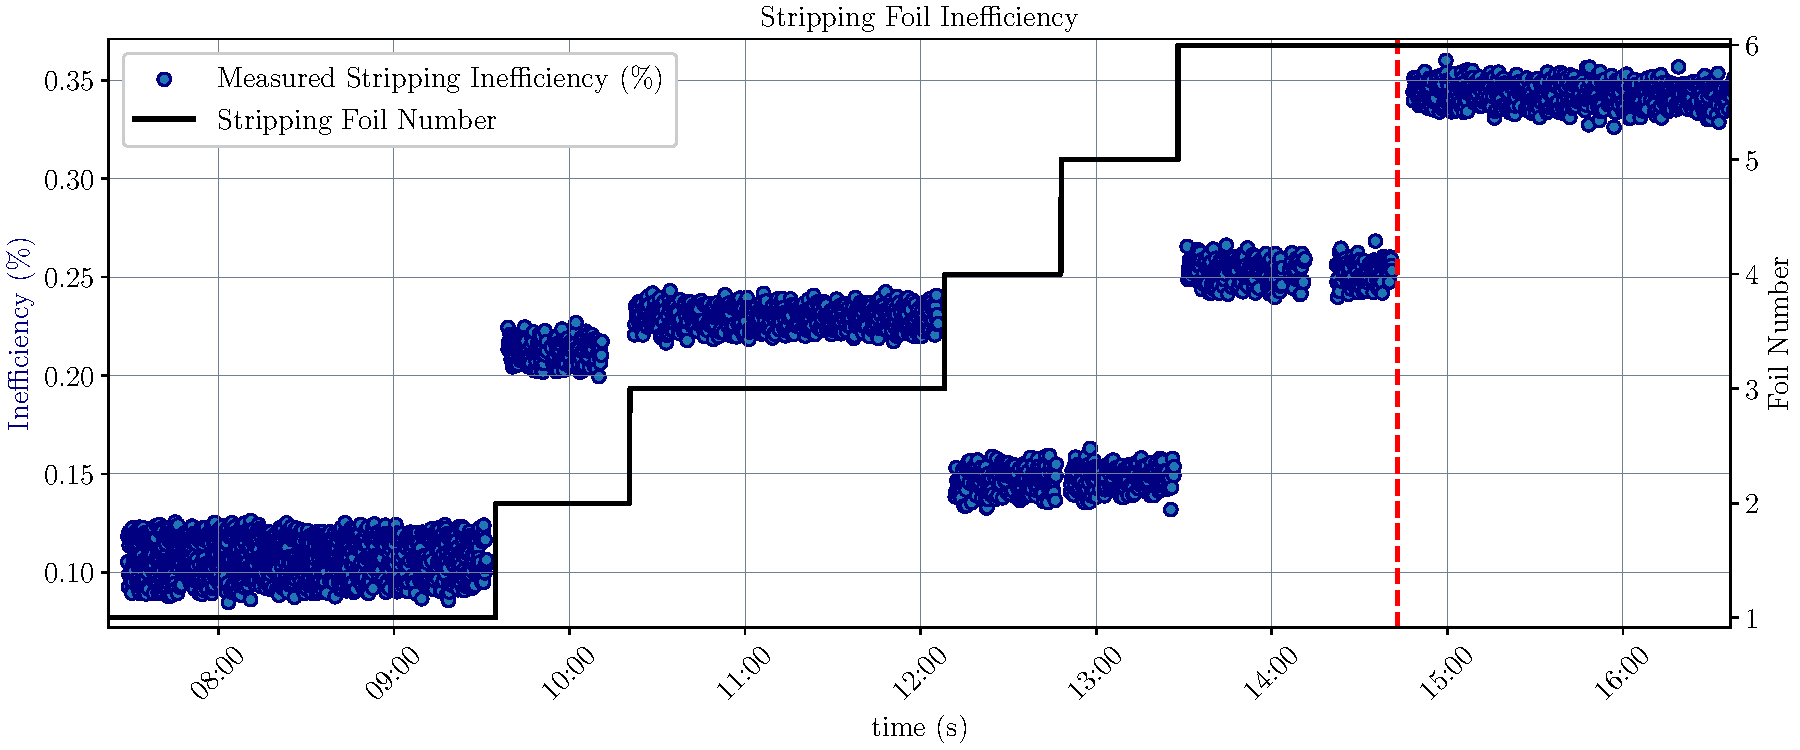
\includegraphics[width=1.0\columnwidth]{StrippingEfficiency13April/April16.pdf}
    \caption{Calculated stripping inefficiency during striping foil tests.}
    \label{fig:StrippingIneff}
\end{figure}

Figure \ref{fig:Histo}, shows a histogram projection of these inefficiency measurements.  The measured stripping inefficiencies are very small, of the order of $0.2 \%$. Even in this situation, the measurement uncertainties are small enough to distinguish between foils. 

Another very interesting feature that could be observed during these tests was the stripping inefficiency increase during foil degradation. A stress test was performed on Foil 6. To determine whether the foil could resist the beam conditions, the beam intensity (bema number of turns) was steadily increased. 

\begin{figure}[h]
    \centering
    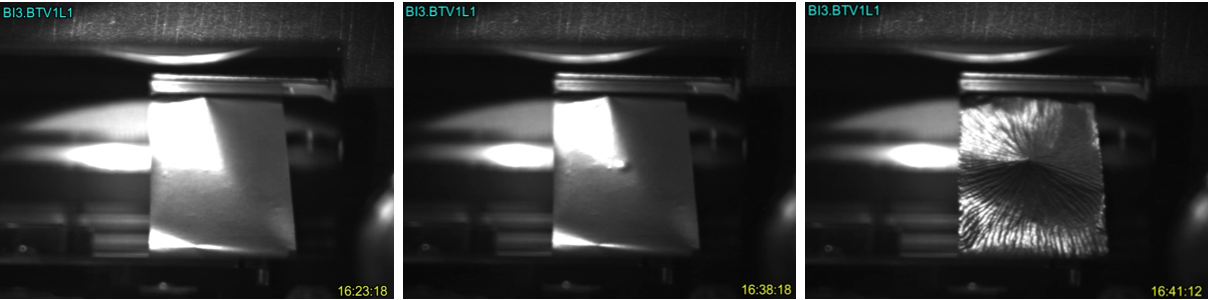
\includegraphics[width=1.0\columnwidth]{Figure_SFPicture/SFDegradationPicture.png}
    \caption{Stripping foil pictures during degradation studies.}
    \label{fig:FoilPicture}
\end{figure}

In picture \ref{fig:FoilPicture} one can observe a picture of the foil at three different stages of the test. The first picture was taken at the beginning of the measurements, and no clear deformation can be observed. The central picture was taken when the injected number of turns was 120. In this case, a small local deformation starts being visible. When 130 beam turns were injected, a sudden deformation occurred, as can be seen in the picture on the right. 

This big deformation could also be observed in the inefficiencies measurements. The red dotted line in figure \ref{fig:StrippingIneff} indicates the exact time when this deformation occurred. The change in the stripping inefficiency is obvious and it can more clearly be observed in \ref{fig:Histo} with the before and after histograms. 

\begin{figure}[h]
    \centering
    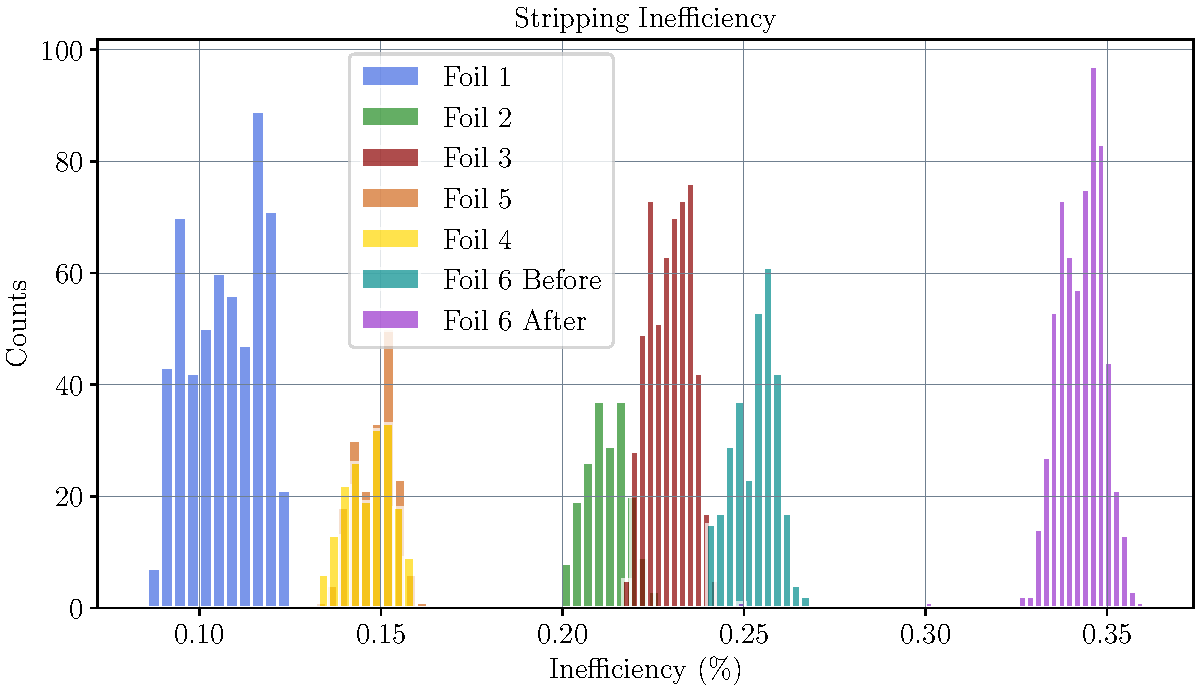
\includegraphics[width=0.75\columnwidth]{StrippingEfficiency13April/Histo.pdf}
    \caption{Histogram representation of the calculated stripping inefficiencies during stripping foil tests. }
    \label{fig:Histo}
\end{figure}

The quantitative values of the stripping foil inefficiencies were subjected to some uncertainties in the measurements, such as beam positioning conditions, possible non-registered beam losses, uncertainties in BCT measurements, etc. For that reason, no quantitative number will be given in this section. Nevertheless, the relative differences between the registered stripping inefficiencies are clear, proving the high sensitivity of the stripping inefficiency measurements. 

\section{Noise Problems}

One of the biggest challenges faced by the \hzhm current monitor was related to electronic interferences. Due to the controlled environments in which the calibration process was carried out, little impact of noise in the signals could be seen. However, during normal operation, a clear presence of electronic noise was observed. Figure \ref{fig:Noise} shows some examples of Plate signal readouts taken in normal operating conditions. 

\begin{figure}[h]
    \centering
    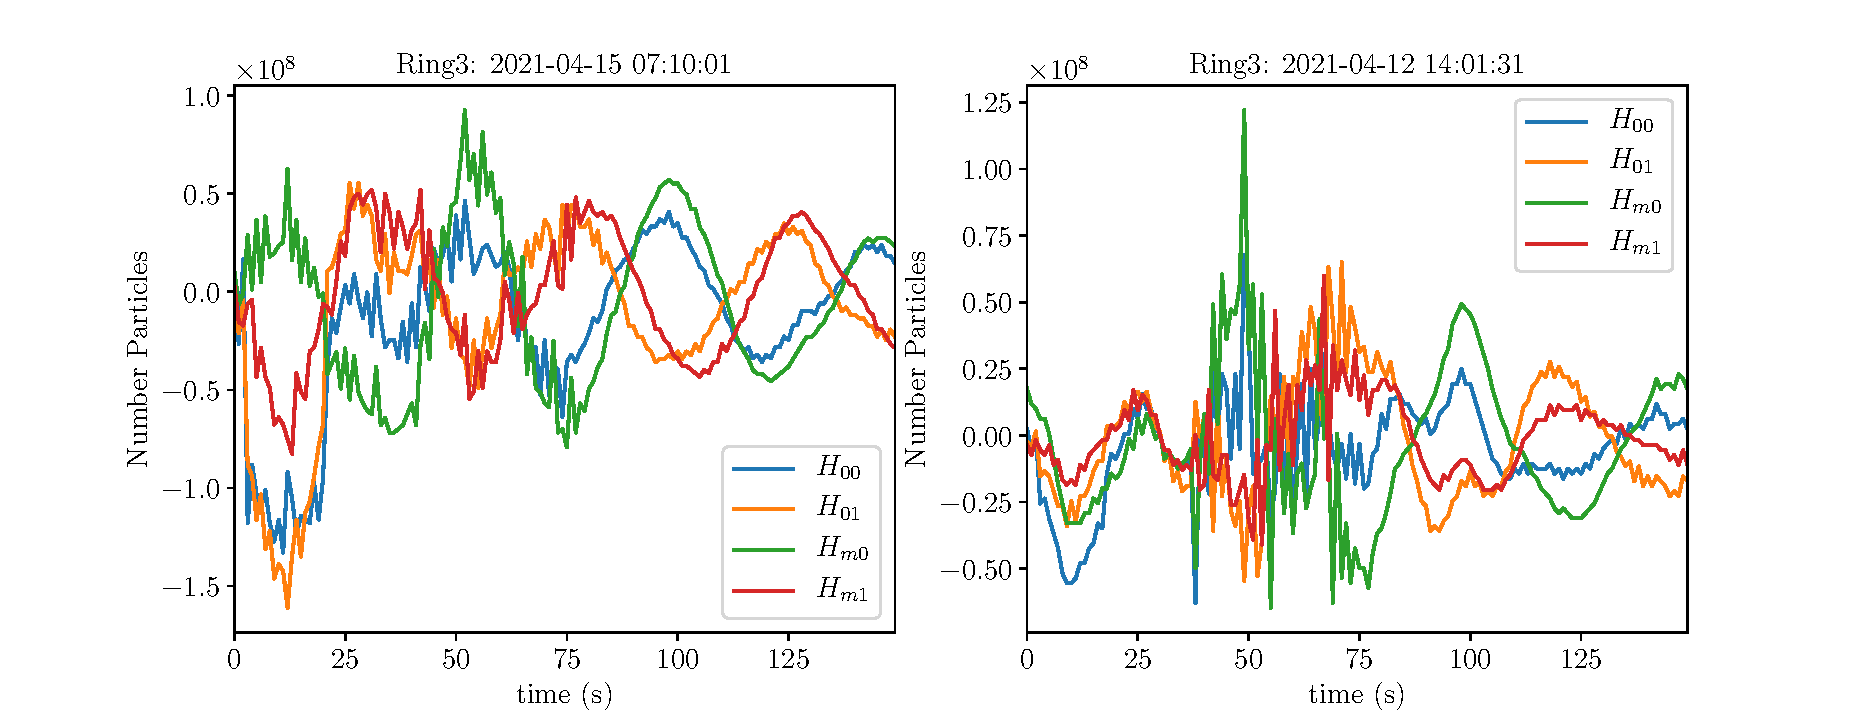
\includegraphics[width=1.0\columnwidth]{Figure_NoiseProblems/NoiseProblem.pdf}
    \caption{Plate signals measured during normal operating conditions. Left: With beam injection. Right: No beam injection. }
    \label{fig:Noise}
\end{figure}

From this figure, one can already see that the noise signals are not negligible. In addition, since the calibration of these detectors in March 2021, several non-physical interlock signals have been reported. These interlocks were attributed to the integration of electronic noise. To avoid these fake interlock signals, it became crucial to minimize the electric noise in our system. Two types of noise were identified, a high-frequency noise and a low-frequency noise. 

\begin{figure}[h]
    \centering
    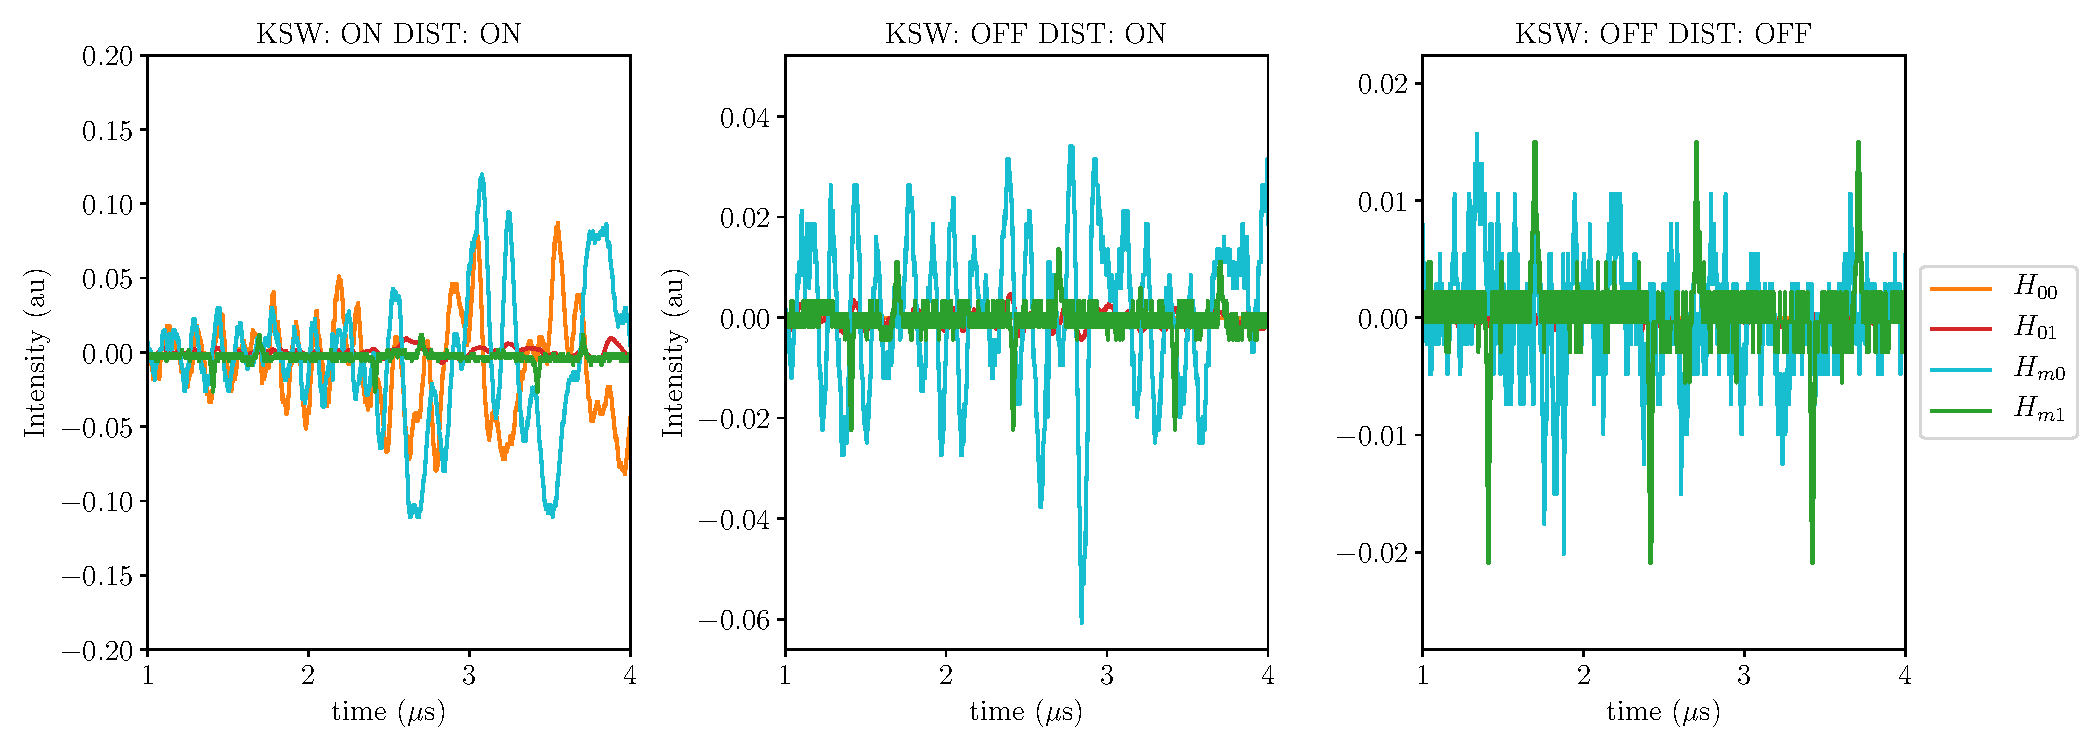
\includegraphics[width=1.0\columnwidth]{Figure_KSWandDISTeffect/KswDistEffect.pdf}
    \caption{Effects of KSW and Distributor in electrical noise signals. Background measurements, no beam. Left: KSW on, Distributor On. Center: KSW off, Distributor Off in the current ring but on in other rings. Right: KSW off, Distributor Off in all rings. }
    \label{fig:KSWandDist}
\end{figure}

\begin{figure}[h]
    \centering
    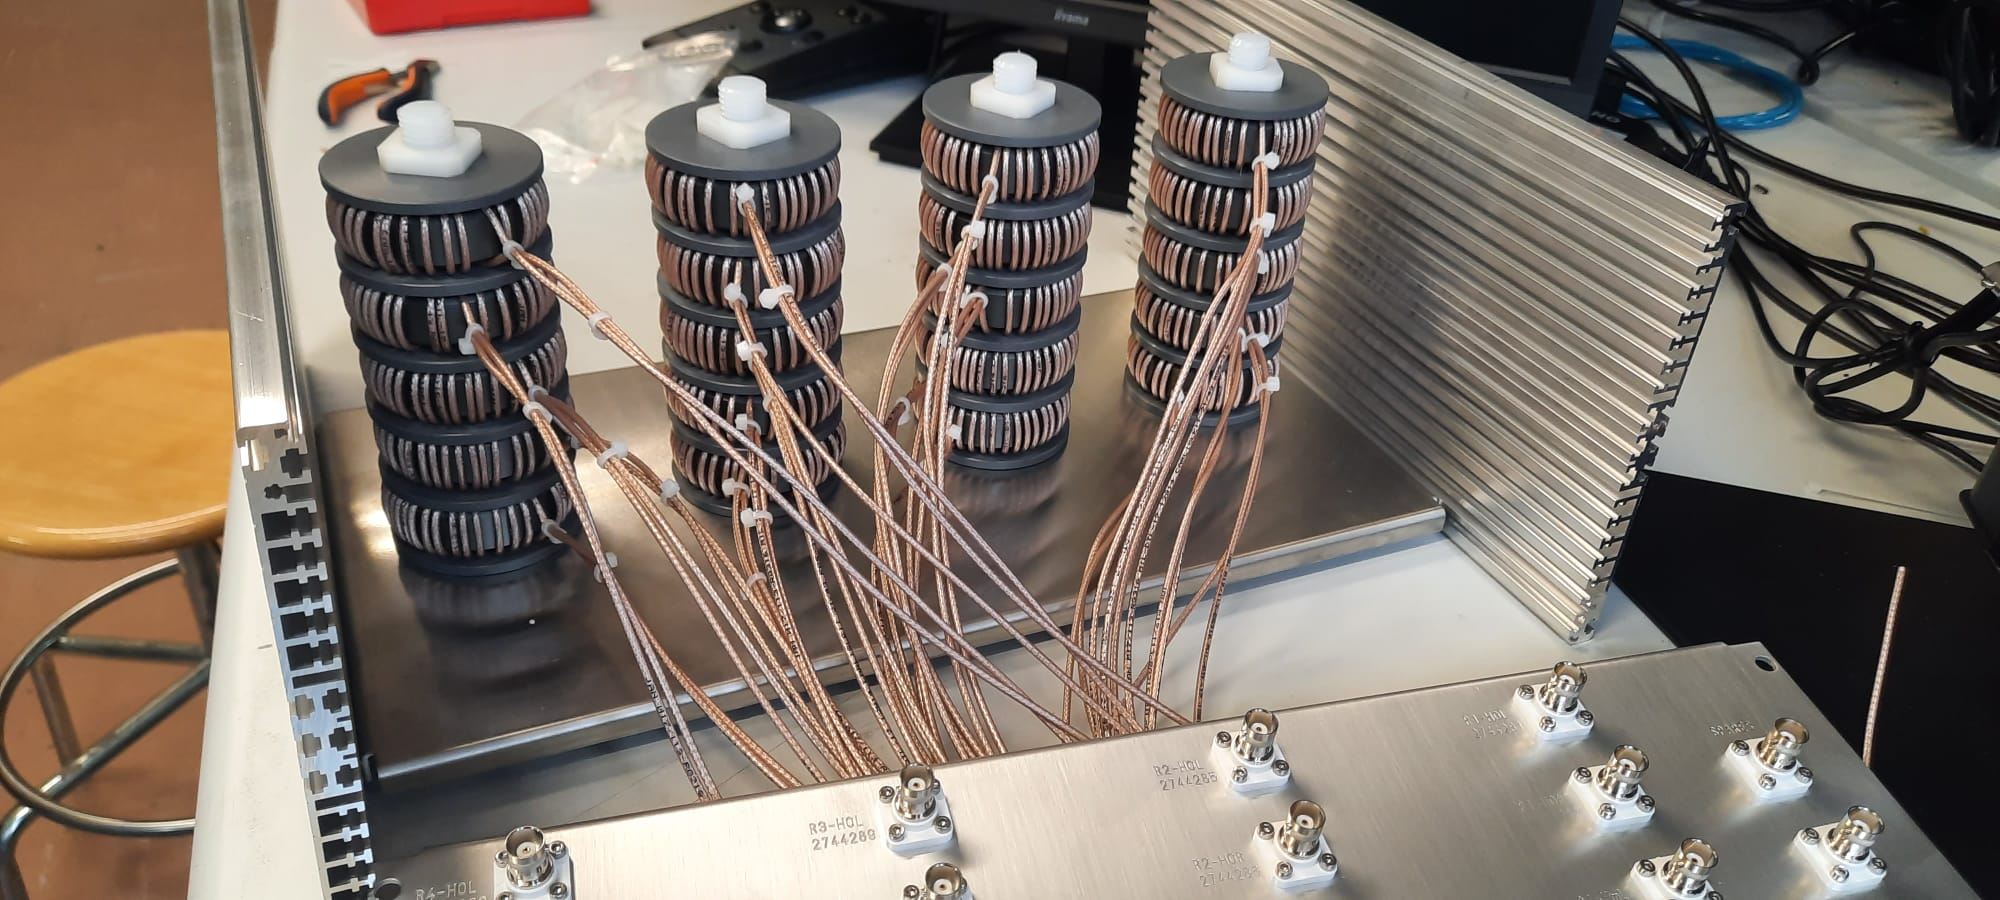
\includegraphics[width=0.8\columnwidth]{Figure_Ferrites/PictureFerrites.jpg}
    \caption{Picture of the ferrites installation for noise mitigation before \hzhm VEME card. }
    \label{fig:Ferrites}
\end{figure}

The high-frequency noise is related to the decaying current of the KSW magnets and the distributor. Figure \ref{fig:KSWandDist} shows the effects these two devices have on the plate signal, where measurements with no beam were taken. It was also observed, that KSWs and distributors of a certain ring were affecting the measurements in other rings. Unfortunately, during normal operation, these devices will always be working, and there is little one can do to improve the generated noise. 


As far as the low-frequency noise is concerned, the origins of the noise are quite unclear. However, thorough investigations were performed to minimize this noise. Ferrites \parencite[][]{ref:Ferrites} were installed at the arrival of the \hzhm beam current monitor signals from the tunnel, just before the VME input. Figure \ref{fig:Ferrites} shows a picture of the installed ferrites. The instalation of these devices improved the noise-signal ratio, as can be seen in figure \ref{fig:BefAftFerrites}. In this figure, the beam conditions for the measurements before and after the ferrite installation were quite different, so the beam signals cannot be directly compared. However, the effects of noise mitigation thanks to the installation of these devices is obvious. 

\begin{figure}[h]
    \centering
    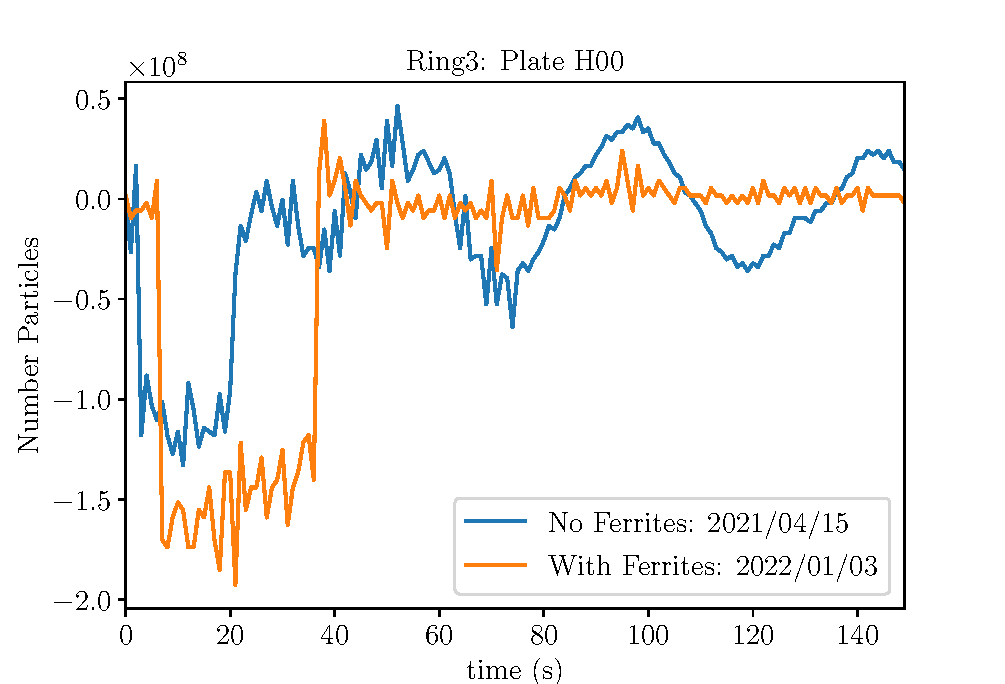
\includegraphics[width=0.7\columnwidth]{Figure_FerritesEffect/BfreAfter.pdf}
    \caption{Effects of the ferrite installation on the \hzhm signals. }
    \label{fig:BefAftFerrites}
\end{figure}
